\documentclass[12pt]{article} 
\usepackage[utf8]{inputenc}

%%% PAGE DIMENSIONS
\usepackage{geometry}
\usepackage{lineno}
\usepackage{color, colortbl}
\usepackage[kernelfbox]{xcolor}
\usepackage{caption}
\usepackage{subcaption}
\usepackage{graphicx}
%%% LANGUAGE HYPHENATION
\usepackage[english]{babel}
%%% HEADERS & FOOTERS
\usepackage{fancyhdr} 
%%% SECTION TITLE APPEARANCE
\usepackage{sectsty}
%%% MATHS RELATED PACKAGES
\usepackage{import}
\usepackage{amsmath}
\usepackage{algorithm}
\usepackage{algpseudocode}
\usepackage{setspace}
\usepackage{array}
\usepackage{multirow}
%%% OTHER PACKAGES
\usepackage{booktabs}
\usepackage{array}
\usepackage{paralist}
\usepackage{verbatim}
\usepackage{subfig}
\usepackage{url}

%%% SETTINGS
\geometry{letterpaper}
\geometry{margin=1in}
\doublespacing
\linenumbers
\allsectionsfont{\sffamily\mdseries\upshape} 
\graphicspath{{./Figures/}}
\pagestyle{fancy}
\renewcommand{\headrulewidth}{0pt}
\lhead{}\chead{Hughes and White -- MODFLOW UPCG GPGPU Solver}\rhead{}
\lfoot{}\cfoot{\thepage}\rfoot{}

\title{Use of general purpose graphical processing units with MODFLOW}
\author{Hughes, J.D.\\U.S. Geological Survey\\ Tampa, Florida\\ \texttt{jdhughes@usgs.gov} \and White, J.T. \\ U.S. Geological Survey\\ Tampa, Florida\\ \texttt{jwhite@usgs.gov}}
%\date{} % Activate to display a given date or no date (if empty),
         % otherwise the current date is printed 

\begin{document}
\maketitle
\begin{abstract}
To evaluate the use of general-purpose graphics processing units (GPGPU) to improve the performance of MODFLOW, an unstructured preconditioned conjugate gradient (UPCG) solver has been developed. The UPCG solver uses a compressed sparse row storage scheme and includes Jacobi, zero fill-in incomplete and modified-incomplete LU factorization, and generalized least-squares polynomial preconditioners. The UPCG solver also includes options for sequential and parallel solution on the central processing unit (CPU) using OpenMP. For simulations utilizing the GPGPU, all basic linear algebra operations are performed on the GPGPU; memory copies between the central processing unit CPU and GPCPU occur prior to the first iteration of the UPCG solver and after satisfying head and flow criteria or exceeding a maximum number of iterations. The efficiency of the UPCG solver for GPGPU and CPU solutions is benchmarked using simulations of a synthetic, heterogeneous  unconfined aquifer with tens of thousands to millions of active grid cells. Testing indicates GPGPU speedups on the order of 2-8, relative to the standard MODFLOW PCG solver, can be achieved when (1) memory copies between the CPU and GPGPU are optimized, (2) the percentage of time performing memory copies between the CPU and GPGPU is small relative to the calculation time, (3) high-performance GPGPU cards are utilized, and (4) CPU-GPGPU combinations are used to execute sequential operations that are difficult to parallelize. Furthermore, UPCG solver testing indicates GPGPU speedups exceed parallel CPU speedups achieved using OpenMP on multi-core CPUs for preconditioners that can be \color{blue}easily \color{black}parallelized.
\end{abstract}

\section*{Introduction}

MODFLOW (Harbaugh 2005) is a finite-difference groundwater flow model that has been effectively applied to \color{blue}numerous \color{black}two- and three-dimensional problems. Because MODFLOW uses a cell-centered finite-difference (CCFD) approximation and a rectilinear grid, model runtimes are often increased by factors of two, four, and eight with increased vertical, horizontal, or combined vertical and horizontal discretization, respectively. \color{blue}Increase model runtimes are typically a direct result of increases in the number of simultaneous equations solved for each cell but can also be affected (typically to a lesser degree) by changes in the coefficient matrix. \color{black}To date, larger model sizes have been accommodated through a combination of faster CPUs and better linear solvers. The original version of MODFLOW (McDonald and Harbaugh 1988) included 1) a strongly implicit procedure (SIP) linear solver and 2) a slice-successive overrelaxation (\color{cyan}SSOR\color{black}) linear solver. These original linear solvers were supplemented with the preconditioned conjugate gradient (PCG2) linear solver (Hill 1990), \color{cyan}the alternating diagonal ordering (DE4) direct solver (Harbaugh 1995), \color{black}the link-algebraic multi-grid (LMG) linear solver (Mehl and Hill 2001), the geometric multigrid (GMG) linear solver (Wilson and Naff 2004), and the  preconditioned conjugate gradient with improved nonlinear control (PCGN) linear solver (Naff and Banta 2008).

Parallelization of linear solvers is another approach for accommodating larger model sizes. \color{blue}Ideal parallelization would result in a linear speedup  (CPU runtime / parallel runtime) as additional CPUs and/or computers were applied to any given problem. For example, if ideal parallelization were achieved and 2, 3, 4, and 5 CPUs were applied to a problem the speedup would be 2, 3, 4, and 5, respectively. However, ideal parallelization is rarely, if ever, achieved because of communication bottlenecks which may be a result of hardware limitations and/or use of algorithms that are difficult to parallelize. \color{cyan}In this study, speedup is calculated using the amount of time spent in solver routines not the total runtime (which includes the time spent in other non-solver routines).\color{black}

\color{black}Dong and Li (2009) parallelized the MODFLOW PCG solver (Hill 1990) using the OpenMP (OpenMP Architecture Review Board, 2005) programming paradigm and observed speedups as large as 5 on machines with multi-core CPUs. Naff (2008) developed a parallelized linear solver for MODFLOW using the Message Passing Interface (MPI) standard and observed a speedup of 7. In addition to OpenMP and MPI, GPGPUs also \color{blue}present \color{black}an option for linear solver parallelization. In comparison to CPUs, GPGPUs \color{blue}typically have more cores (\textit{e.g.}, 448 cores in the case of the NVIDIA$^{\textregistered}$ Tesla™ C2050 and C2070 GPGPUs), have higher bandwidth, and as a result are capable of executing more floating point operations per second. \color{black}Use of GPGPUs to parallelize linear solvers for MODFLOW is also attractive because of the availability of the CUDA (Compute Unified Device Architecture) application programming interface (API) for NVIDIA GPGPUs, which supports development of parallel GPGPU code in C/C++ or Python, Fortran, Java, and MATLAB using wrappers around the C/C++ implementation. For example, Soni \textit{et al.} (2012) used the CUDA language to develop a GPGPU code to solve computational fluid dynamics problems. For solution of the groundwater flow equation, Ji \textit{et al.} (\color{cyan}2010 and \color{black}2012) developed a parallel GPGPU version of MODFLOW-2000 with a Jacobi preconditioner and observed speedups ranging from 1.8 to 3.7.

In this paper, we evaluate speedups resulting from GPGPU parallelization of the unstructured UPCG linear solver for a unconfined groundwater flow problem. We also evaluate the performance of the UPCG linear solver using Jacobi, zero fill-in modified incomplete LU (MILU0), and generalized least-squares polynomial (GLSPOLY) preconditioners on the CPU and GPGPU. And finally, we evaluate the performance of the UPCG solver on the GPGPU to parallel CPU simulations using the OpenMP parallel programming paradigm.

\section* {\bf GPGPU Parallel Programming}
GPGPU code developed using the NVIDIA$^{\textregistered}$ CUDA API is essentially a sequential code that is capable of using the fork-join model of parallel execution similar to OpenMP. In a fork-join model, a single master thread is active when program execution begins. The master thread executes sequential portions of the code. At points where parallel operations are required, the master thread spawns, or forks, additional threads that work concurrently with the master thread through the parallel section. At the end of the parallel code, the spawned threads are suspended and rejoined to the master thread. The fork-join model used in OpenMP is shown graphically in \textbf{figure~\ref{FigParallel}}. Typically, the number of OpenMP threads used in the fork-join model is less than the total number of cores available on multi-core CPUs.

For GPGPU code implementations, the concept is similar to OpenMP.  The main code is a sequential host code which forks the data into many threads at the invocation of a CUDA \color{blue}functions, called kernels (\textbf{Box 1})\color{black}.  \color{blue}However, as opposed to the few threads spawned by OpenMP, GPGPUs have to potential to spawn thousands to tens-of-thousands of threads to execute the CUDA kernel function (\textbf{Box 2}). The NVIDIA Tesla C2050 used to evaluate the UPCG solver in this study can execute 21,504 concurrent threads. \color{black} With thread counts on the order of tens of thousands, GPGPUs have great potential for parallelization \color{blue} for MODFLOW and other numerical simulators that use Krylov subspace methods to solve large systems of simultaneous linear equations\color{black}.


\section* {\bf Conjugate Gradient Linear Solver}
The constant-density, three-dimensional groundwater flow equation is described by the partial-differential equation,

\begin{equation}
	\label{gwpde}
	\frac{\partial}{\partial x} \left( K_{xx} \frac{\partial h}{\partial x} \right) + 
	\frac{\partial}{\partial y} \left( K_{yy} \frac{\partial h}{\partial y} \right) + 
	\frac{\partial}{\partial z} \left( K_{zz} \frac{\partial h}{\partial z} \right) + 
	W = S_{S} \frac{\partial h}{\partial t} ,
\end{equation}

\noindent
where  $K_{xx}$, $K_{yy}$, $K_{zz}$ are the hydraulic conductivity [L/T] along the x, y, and z-coordinate axes which are assumed to be parallel to the major axes of hydraulic conductivity; $h$ is the groundwater head [L]; $W$ is a volumetric flux per unit volume [L$^{3}$/L$^{3}$T] representing sources/sinks of water; S$_{S}$ is the specific storage [L$^{-1}$]; and t is time [T].

MODFLOW uses a cell-centered, finite-difference approximation of \textbf{equation~\ref{gwpde}} to solve for three-dimensional groundwater flow (Harbaugh 2005). Development of the finite-difference form of \textbf{equation~\ref{gwpde}} using the continuity equation for a cell results in

\begin{equation}
	\label{conteq}
	\sum Q = S_{S} \frac{\Delta h}{\Delta t} V,
\end{equation}

\noindent
where $Q$ is the flow rate [L$^{3}$/T] into a cell from adjacent cells and sink/source terms, $\Delta h$ is the head change [L] in a cell over a time interval $\Delta t$ [T], and $V$ is the volume of a cell [L$^{3}$]. Manipulation of \textbf{equation~\ref{conteq}} to separate known and unknown $h$ terms results in a large system of simultaneous linear equations of the form, 

\begin{equation}
	\label{lineareq}
	\mathbf{Ah} = \mathbf{b},
\end{equation}

\noindent
where $\mathbf{A}$ is a  square, symmetric, positive-definite coefficient matrix [L$^{2}$/T] that includes cell-by-cell conductances, calculated using cell dimensions and hydraulic conductivities at cell interfaces, and unknown components of sink/source and storage terms; $\mathbf{h}$ is the vector of unknown heads at time $t$; and $\mathbf{b}$ is a known vector of source/sink and storage terms.

\subsection*{Conjugate Gradient Algorithm}

The conjugate gradient (CG) iterative method is an efficient method for solving large systems of linear equations having a square, symmetric, positive-definite coefficient matrix. Pseudocode for the preconditioned conjugate gradient method is given in \textbf{algorithm~\ref{pcgalg}}. 

\begin{algorithm}
\caption{Preconditioned Conjugate Gradient Method}
\label{pcgalg}
\begin{algorithmic}[1]
	\State $\text{Compute } \mathbf{r}_{0} = \mathbf{b - Ah}_{0} \text{ for some initial guess } \mathbf{h}_{0}$
	\For {$i = 1 \to maxinner$}
		\State $\textbf{solve } \mathbf{Mz}_{i-1} = \mathbf{r}_{i-1}$ \Comment{apply preconditioner}
		\State $\rho_{i-1} = \mathbf{r}^T_{i-1} \mathbf{z}_{i-1}$
		\If {$i = 1$}
			\State $\mathbf{p}_i = \mathbf{z}_0$
		\Else
			\State $\beta_{i-1} = \rho_{i-1} / \rho_{i-2}$
			\State $\mathbf{p}_i = \mathbf{z}_{i-1} + \beta_{i-1} \mathbf{p}_{i-1}$
		\EndIf
		\State $\mathbf{q}_i = \mathbf{Ap}_{i}$
		\State $\alpha_i = \rho_{i-1} / \mathbf{p}^T_i \mathbf{q}_{i}$ \Comment{calculate step-size}
		\State $\mathbf{h}_i = \mathbf{h}_{i-1} + \alpha_i \mathbf{p}_{i}$  \Comment{update head}
		\State $\mathbf{r}_i = \mathbf{r}_{i-1} - \alpha_i \mathbf{q}_{i}$ \Comment{update residual}
		\State $\text{check convergence; continue if necessary}$
	\EndFor
\end{algorithmic}
\end{algorithm}

In \textbf{algorithm~\ref{pcgalg}}, $\mathbf{r}$ is the \color{cyan}difference between the left and right side (residual) \color{black}of \textbf{equation~\ref{lineareq}} [L$^3$/T], $i$ is the linear iteration index [unitless], $maxinner$ is a user-specified maximum number of iterations to perform [unitless], $\mathbf{M}$ is the preconditioned form of $\mathbf{A}$ [L$^2$/T], $\mathbf{z}$ is the solution resulting from application of $\mathbf{M}$ to $\mathbf{r}$ [L$^3$/T], $\mathbf{p}$ is the orthogonal search direction [L], $\beta$ is a scalar used to determine the next search direction [unitless], $\mathbf{q}$ is the residual change resulting from multiplication of $\mathbf{A}$ and the search direction $\mathbf{p}$ [L$^3$/T], $\alpha$ is the step-size [unitless]. \color{cyan}Readers are referred to Barrett \textit{et al.} (1994) for more information on the PCG method.\color{black}

All linear iteration steps, except for application of the zero fill-in incomplete LU (ILU0) and MILU0 preconditioners in line 3 of \textbf{algorithm~\ref{pcgalg}}, include operations that are independent for each active groundwater cell, indicating a potential for parallelization. In cases where (1) no preconditioner ($\mathbf{z = r}$) or (2) a Jacobi preconditioner ($\mathbf{M = I D}^{-1}$ -- where $\mathbf{I}$ is the identity matrix and $\mathbf{D}^{-1}$ is a matrix that only contains the inverse of the diagonal elements of $\mathbf{A}$), is selected, application of the preconditioner is highly parallelizable. For most practical problems, non-preconditioned and the Jacobi preconditioners will not significantly reduce the number of linear iterations ($i$) required to achieve convergence (Li and Saad 2010). As a result better preconditioners, such as incomplete factorizations (ILU0 or MILU0) or m-degree polynomial (GLSPOLY) approximations of $\mathbf{A}$, are generally needed. Application of the incomplete factorization preconditioners requires a forward substitution ($\mathbf{Ly = b}$ -- where $\mathbf{L}$ is the lower triangular portion of $\mathbf{A}$) followed by a backward substitution ($\mathbf{Uz = y}$ – where $\mathbf{U}$ is upper triangular portion of $\mathbf{A}$) and is difficult to efficiently parallelize (Barrett \textit{et al.} 1994). Preconditioning using polynomial preconditioners, however, is simple, efficient, and very easy to parallelize \color{cyan}because polynomial preconditioner application only requires a limited number matrix-vector product and a constant times a vector plus a vector (axpy) BLAS operations \color{black} (Liang \textit{et al.} 2002; Saad 2003).

\subsection*{Numerical Implementation}
The UPCG linear solver was coded to allow solution of the groundwater flow equation on either the CPU, GPGPU, or combination of CPU and GPGPU using double precision operations. Execution of the UPCG solver on the CPU, GPGPU, or combination of CPU and GPGPU is specified by the user in the UPCG input file.

Although the connectivity of the finite-difference discretization used in MODFLOW uses a fixed 5- and 7-point stencil in two- and three-dimensions, respectively, the PCG method in \textbf{algorithm~\ref{pcgalg}} was coded using an unstructured compressed sparse row storage (CSR) format  (Barrett \textit{et al.} 1994) with the diagonal element in the first position in each row. This storage format is also supported by the \color{blue}CUDA-enabled implementation of the BLAS library (CUBLAS -- NVIDIA 2012). BLAS is a library of Basic Linear Algebra Subprograms (Lawson \textit{et al.} 1979)\color{black}. The UPCG linear solver includes Jacobi, ILU0, MILU0, and GLSPOLY preconditioners (\color{cyan}Saad \color{black}2003).

Available CUBLAS matrix-vector products and level-1 BLAS operations were used to parallelize the GPGPU capabilities of the UPCG linear solver. Because of the poor performance of forward and back substitution operations used by the ILU0 and MILU0 preconditions observed during initial testing of the UPCG linear solver and observed by others (Li and Saad 2010), application of these preconditioners is performed on the CPU, resulting in a hybrid CPU/GPGPU solver. The results of the matrix-vector product, calculated by application of the ILU0 and MILU0 preconditioners on the CPU, is accessed as page locked memory by the GPGPU to achieve higher memory bandwidth.

For parallel CPU simulations, OpenMP directives were added to all matrix-vector products and level-1 BLAS operations. The OpenMP matrix-vector product was constructed using a level-2 BLAS \color{cyan}general matrix-vector (GEMV) product \color{black}approach because of the slight increase in performance of this approach over dot-product and \texttt{axpy} approaches for calculating matrix vector products (Petersen and Arbenz 2004). OpenMP directives \texttt{NUM\_THREADS} and \texttt{SCHEDULE STATIC} were used in all OpenMP routines to allow the user to control the number of OpenMP threads and reduce OpenMP scheduling/synchronization overhead, respectively. The number of OpenMP threads used for matrix-vector products and level-1 BLAS operations is specified separately in the UPCG input file. For sequential CPU simulations,  separate matrix-vector product and level-1 BLAS operation routines that exclude OpenMP directives are used to eliminate all OpenMP overhead.

Infinity norms ($\left \|  x \right \|_{\infty}$) are used to evaluate convergence of the UPCG linear solver with respect to the change in $\mathbf{h}$ (HCLOSE) and $\mathbf{r}$ (RCLOSE). In MODFLOW, non-linearities are resolved using Picard iteration. Picard iteration is implemented such that the $\mathbf{A}$ matrix is formulated using the latest estimate of $\mathbf{h}$, then $\mathbf{h}$ and $\mathbf{r}$ are updated using a linear solver. This process is continued until the maximum change in $h$ and $r$ in any model cell is less than HCLOSE and RCLOSE, respectively, on the first iteration ($i$=1) of the linear solver or the maximum number of Picard (outer) iterations is exceeded; \color{cyan}the UPCG solver approach for evaluating convergence is identical to the standard MODFLOW PCG solver (Hill 1990).\color{black}


\section* {\bf Test Cases}
The performance of the GPGPU implementation of the UPCG linear solver was evaluated on a NVIDIA Tesla C2050 GPGPU with 3 GB of RAM and capable of 515 GFLOP/sec of double precision processing performance (NVIDIA compute capability 2.0). The GPGPU was mounted in a 16-pin PCI local bus on a single quad core Intel \color{cyan}Xeon \color{black}3GHz CPU, capable of executing 4 threads per CPU, with 6 GB of RAM and running a 64-bit version of the Windows 7 Enterprise OS. For comparison with GPGPU results, \color{cyan}serial and \color{black}parallel CPU simulations were executed on dual 4-core Intel \color{cyan}Xeon \color{black}2.4 GHz CPUs, capable of executing 8 parallel threads, with 16 GB of RAM running a 64-bit version of the Windows Server 2008 R2 Standard OS (Service Pack 1).

\color{blue}To evaluate the performance of the GPGPU implementation of the UPCG linear solver a  synthetic test problem with aquifer properties and boundary conditions that result in equivalent problems and scalable runtimes if discretized using different horizontal and vertical cell sizes. The test problem represents an unconfined aquifer to increase the difficulty of the problem by making it non-linear as a result of the dependence of the $\mathbf{A}$ matrix in \textbf{equation~\ref{lineareq}} on the solution of $\mathbf{h}$. Furthermore, the test problems used realistic initial conditions sufficiently far from final results to start with an incorrect $\mathbf{A}$ matrix to maximize (1) head changes during solution of the problem and (2) the number of Picard iterations required to achieve a solution.\color{black}

\subsection*{Problem Description}
GPGPU and parallel CPU results were evaluated using a number of horizontal and vertical model discretizations of a 1,000 m square heterogeneous unconfined aquifer. The top and bottom of the aquifer are flat and specified to have elevations of 10 and -30 m, respectively. Models with horizontal discretizations of 200 $\times$ 200, 500 $\times$ 500, 1,000 $\times$ 1,000, 2,000 $\times$ 2,000, and 4,000 $\times$ 4,000 cells per layer were evaluated. Single layer models were evaluated for all horizontal discretizations and multi-layer models were evaluated for select horizontal discretizations to determine the effect that a 7-point stencil, and the resulting additional non-zero entries for each cell, has on GPGPU and parallel CPU execution time. Two- and three-layer models were evaluated for all horizontal discretizations except 4,000 $\times$ 4,000 cells per layer. Ten-layer models were also evaluated for horizontal discretizations ranging from 200 $\times$ 200 to 1,000 $\times$ 1,000 cells per layer. Additional horizontal and vertical discretizations were not evaluated because of GPGPU memory requirements for larger problems. For multi-layer models, a constant layer thickness was used for all but the first layer and was calculated by dividing 30 m by the number of layers. \color{blue}Layer 1 also includes the thickness of the aquifer above the arbitrary elevation of 0 m and therefore is 10 m thicker than layer 2.\color{black}

The heterogeneous hydraulic conductivity distribution (base hydraulic conductivity data) was generated for the 1,000 $\times$ 1,000 cell model (base model) using sequential Gaussian simulation with log-transformed (base 10) parameters based on a mean value of 5 m/d and an exponential variogram having a nugget of 1.023 $\log_{10}((m/d)^{2})$, a variance of 1.23 $\log_{10}((m/d)^{2})$, and length parameter ($a$) of 250.5 m (effective range $\approx$ 750 m). The axis of anisotropy was rotated by 45 degrees to the model grid and a 3.5:1 ratio of horizontal anisotropy was used. For the realization selected and used to evaluate GPGPU and parallel CPU results, the minimum, average, and maximum hydraulic conductivity in the model domain were 0.43, 4.81, and 43.3 m/d, respectively. The distribution of hydraulic conductivity in the model domain is shown in \textbf{figure~\ref{FigModelDomain}}.

Hydraulic conductivity was not varied between layers in the multi-layer models evaluated. For models having less than 1,000 $\times$ 1,000 cells per layer, the base hydraulic conductivity data was averaged for each base model cell contained in a coarse model cell. For models having more than 1,000 $\times$ 1,000 cells per layer, the base hydraulic conductivity data was directly assigned to each higher-resolution cell contained within a coarse base model cell.

Head-dependent (general head) boundaries were specified on the left and right sides \color{cyan} in all layers \color{black} and no flow boundaries at the top and bottom. Head-dependent boundaries are assumed to be located a half model cell away from the edge of the model domain and conductance values were calculated using the average hydraulic conductivity of 4.81 m/d, vertical saturated cell areas, and half the model cell dimensions in the x-direction; head-dependent boundary head values were calculated using the hydraulic gradient over the model domain \color{blue}$\left [ 10. / 1000. = 0.01 \text{ m/m} \right]$ \color{black}and assumed heads at the left and right sides of the model domain of 10.0 and 0.0 m, respectively. For the one layer 1,000 $\times$ 1,000 cell model, conductance and head values of 214.1447 m$^{2}$/d, 160.6085 m$^{2}$/d, 10.025 m, and -0.025 m were specified for the left and right side of the model domain, respectively. The head-dependent boundaries cause an ambient groundwater flow from left to right. Four pumping wells, located in the four cells in the center of the model domain, pump at a constant rate with a total groundwater withdrawal rate of 1,000 m$^3$/d \color{cyan}and represents 46\% of the flow entering the model\color{black}. For multi-layer simulations, the pumping wells withdraw water from the lower model layer. There is no recharge or evapotranspiration; all groundwater flow to the wells is provided by the head-dependent boundaries. Boundary conditions are shown graphically in \textbf{figure~\ref{FigModelDomain}}.

For all model discretizations, the UPCG solver with the Jacobi, MILU0, and GLSPOLY preconditioners were evaluated on the CPU, using both the sequential and parallel (OpenMP) options, and GPGPU. To maximize the amount of time spent in the linear solvers the maximum number of Picard and inner (linear) iterations were set to 50 and 1,000, respectively. A HCLOSE value of 0.001 m was used for all simulations. In order to use a consistent RCLOSE value in all simulations, RCLOSE was calculated as the product of HCLOSE and the cell area, effectively scaling RCLOSE with the discretization. A degree 10 polymonial was constructed for simulations using the GLSPOLY preconditioner and because the coefficient matrix $\mathbf{A}$ was scaled using diagonal scaling we assumed the minimum and maximum eigenvalues for the scaled matrix were between 0.0 and 2.0 (Scandrett 1989).

All of the models simulated steady-state conditions. As a result, specific storage and specific yield values were not specified for the aquifer. Initial heads were specified to be 0.0 m throughout the model domain, sufficiently different from final steady-state heads. Simulated heads \color{cyan} that satisfy specified convergence criteria \color{black} for the one layer 1,000 $\times$ 1,000 cell model are shown in \textbf{figure~\ref{FigModelDomain}} and show the effect that groundwater withdrawals and heterogeneous hydraulic conductivity have on water levels. \color{cyan}Simulated water-levels for simulations that satisfy specified convergence criteria and use different (1) solvers, (2) preconditioners, and/or (3) hardware are within $\pm$RCLOSE m.\color{black}

\subsection*{Results}
\color{blue}The number of Picard and inner iterations required to solve the test problems on the CPU are summarized on \textbf{table~\ref{TableCPUITSummary}}; the number of Picard and inner iterations required to solve the test problems on the GPGPU and the combination of the GPGPU and CPU were identical to the number required on the CPU. The number of Picard and inner iterations required by the MILU0 preconditioner is comparable to the standard MODFLOW PCG solver with the modified incomplete Cholesky (MIC) preconditioner (Hill 1990). The number of Picard iterations is also comparable between the MILU0, PCG solver with the MIC preconditioner, and the GMG solver with the ILU0 preconditioner; the GMG inner iterations are not comparable because of the differences in the inner iteration approaches of both the UPCG and PCG solvers and the GMG solver. The number of Picard and inner iterations required by the GLSPOLY preconditioner generally exceeds the MILU0 preconditioner and the PCG solver with the MIC preconditioner by a factor of but it is notably better the Jacobi preconditioner. In fact, the maximum number of Picard and inner (linear) iterations were exceeded for the 4,000 $\times$ 4,000 $\times$ 1 cell problem simulated using the Jacobi preconditioner, highlighting that the Jacobi preconditioner is not a robust preconditioner for some problems.\color{black}

The CPU/GPGPU speedup of UPCG solver simulations for the Jacobi, MILU0, and GLSPOLY preconditioners are summarized on \textbf{table~\ref{TableGPUCPUSpeedup}}. Significant  CPU/GPGPU speedups, ranging from 1.5 to 35, are observed with Jacobi and GLSPOLY preconditioners. Only marginal speedups, ranging from less than 1.0 to almost 2.0, are observed with the MILU0 preconditioner. The smallest CPU/GPGPU speedup corresponds with the smallest model discretizations (200 $\times$ 200 $\times$ 1) because of the overhead associated with GPGPU-CPU memory copy operations relative to the solution time. 
 
The CPU/GPGPU speedup of MILU0 and GLSPOLY simulations are shown graphically on \textbf{figure~\ref{FigCPUGPUResults}}. The CPU/GPGPU speedup of MILU0 simulations are approximately 2 for simulations with more than 3 million active model cells. The reduction in the CPU/GPGPU speedup of MILU0 simulations between 1 and 3 million active model cells is a result of the higher percentage of runtime spent transferring preconditioner data ($\mathbf{r \text{ and } z}$ in \textbf{algorithm~\ref{pcgalg}}) between the GPGPU and CPU during each linear iteration for application of the MILU0 preconditioner. The CPU/GPGPU speedup of  GLSPOLY preconditioner increases to approximately 30 for simulations with more than 5 million active cells; the increase in the CPU/GPGPU speedup with increased problem size for the Jacobi preconditioner is comparable to the GLSPOLY preconditioner (\textbf{fig.~\ref{FigCPUGPUResults}b}).

The amount of time applying the MILU0 and GLSPOLY preconditioners, performing matrix-vector operations, level-1 BLAS operations, and transferring data between the CPU and GPU for a select number of simulations are shown graphically in \textbf{figure~\ref{FigBLASOperationResults}}. Matrix-vector operations account for approximately half of the time spent in the UPCG solver for sequential CPU simulations using either the MILU0 or GLSPOLY preconditioners. On the GPGPU, matrix-vector operations for the MILU0 and GLSPOLY preconditioner are significantly reduced, largely as a result of the ability of the GPGPU to apply massively parallel resources to perform BLAS operations.  Analysis of operation execution times indicates that the MILU0 speedup is notably less than the GLSPOLY speedup because the time spent applying the MILU0 is essentially the same whether the GPGPU is used or not.  This is because the application of the MILU0 preconditioner is always performed on the CPU.  For the MILU0 preconditioner, all of the speedup occurs during the conjugate gradient routine in the level-1 BLAS operations [matrix-vector multiplication and vector operations (dot products)], which are carried out on the GPGPU after application of the preconditioner. Furthermore, because of additional memory transfers between the CPU and GPGPU when using the MILU0 preconditioner, the total time spent applying the preconditioner actually increases \color{cyan}(\textbf{fig.~\ref{FigBLASOperationResults}a} and \textbf{b})\color{black}. For the GLSPOLY preconditioner, solution on the GPGPU reduces the time spent completing linear solver operations by more than 95\% and the time spent transferring data between the CPU and GPGPU is negligible.
 

\section* {\bf Discussion}
Although notable, CPU/GPGPU speedups summarized on \textbf{table~\ref{TableGPUCPUSpeedup}} are not a fair measure of the speedups that would result from use of the GPGPU to solve a MODFLOW problem. A more realistic comparison is the speedup of GPGPU simulations relative to sequential CPU simulations using the standard MODFLOW PCG solver with the MIC preconditioner (Hill 1990). PCG(MIC)/GPGPU speedups for the Jacobi, MILU0, and GLSPOLY preconditioners are summarized on \textbf{table~\ref{TableGPUSpeedup}}.  PCG(MIC)/GPGPU speedups for the MILU0 and GLSPOLY preconditioners are shown graphically on \textbf{figure~\ref{FigGPUResults}}. 

PCG(MIC)/GPGPU speedups for the MILU0 preconditioner are comparable to CPU/ GPGPU speedups; the similarity of PCG(MIC)/GPGPU and CPU/GPGPU speedups for the MILU0 preconditioner are a result of the similarity in time required to perform forward and backward substitutions during application of the preconditioner with the PCG and UPCG solvers, as the MIC is similar to MILU0 . PCG(MIC)/GPGPU speedups for the Jacobi and GLSPOLY preconditioners range from less than 1.0 to more than 8.0, which are notably less than CPU/GPGPU speedups.  \color{cyan}Reduced PCG(MIC)/GPGPU speedups for the Jacobi and GLSPOLY preconditioners relative to CPU/GPGPU speedups can be attributed to the general efficiency of the MODFLOW PCG solver that is a result of serial coding to reduce solver memory requirements. \color{black}The relative increase in PCG(MIC)/GPGPU speedups \color{cyan}observed for larger problems with \color{black}the Jacobi and GLSPOLY preconditioners is a result of the reduced efficiency of the PCG solver with the MIC preconditioner as the number of model layers increase (\textbf{fig.~\ref{FigGPUResults}b}).

Parallel CPU simulations were run to compare speedups possible with GPGPUs to speedups that could be realized on multi-core CPUs using the OpenMP programming paradigm. \color{blue} The PCG solver parallelized by Dong and Li (2009) using OpenMP was not evaluated in this study because we wanted to directly compare CPU, GPGPU, and parallel CPU runtimes for the same solver. \color{black}PCG(MIC)/UPCG-OpenMP speedups for the Jacobi, MILU0, and GLSPOLY preconditioners using 4, 7, and 14 OpenMP threads are summarized on \textbf{table~\ref{TableOpenMPSpeedup}}. PCG(MIC)/UPCG-OpenMP speedups for the Jacobi and GLSPOLY preconditioners are notably less than PCG(MIC)/GPGPU speedups and is expected because the number of threads on the GPGPU is orders of magnitude greater than for parallel CPU simulations. \color{cyan} In some cases, PCG(MIC)/UPCG-OpenMP speedups are less than 1 as a result of the limited number of threads available and the numerical overhead associated with managing OpenMP threads. \color{black}For the MILU0 preconditioner, PCG(MIC)/UPCG-OpenMP speedups (average speedup $=$ 1.539) are comparable to PCG(MIC)/GPGPU speedups (average speedup $=$ 1.447) and there is little benefit to using the GPGPU with the MILU0 preconditioner. PCG(MIC)/UPCG-OpenMP speedups for the MILU0 preconditioner with 7 OpenMP threads are shown graphically on \textbf{figure~\ref{FigOpenMPResults}}. It should be noted that the Intel Fortran compiler (version 12.1.2.278), with the highest-level optimization option (/O3 compiler switch), was used to compile MODFLOW with the UPCG solver. The relatively small PCG(MIC)/UPCG-OpenMP speedups observed with the UPCG solver compiled using the Intel Fortran compiler is consistent with the observations of Dong and Li (2009). \color{blue} We observed similar PCG(MIC)/UPCG-OpenMP speedups with and without optimization of the executable compiled by the Intel Fortran compiler.\color{black}

\color{blue}Based on our results we believe we can offer the following suggestion regarding use of parallel strategies on GPGPUs and CPUs: (1) in cases where the GLSPOLY preconditioner is adequate, solution on the GPGPU will result in significant speedup over serial and parallel CPU solutions; (2) in some cases the use of the Jacobi preconditioner will result in a GPGPU speedup that exceeds the speedup possible with other preconditioner options but this will be the exception rather than the rule and only applicable to select problems (and likely very simple problems); (3) in cases where a stronger preconditioner than the GLSPOLY preconditioner is required, the parallel CPU version of the MILU0 preconditioner will result in the largest speedup; and (4) in cases with smooth, low-frequency error components a completely different solver, such as the LMG or GMG solver, may be needed (see Mehl and Hill 2001). The effectiveness of a preconditioner will be based on the distribution of the eigenvalues of the preconditioned matrix. For some problems the eigenvalues of the Jacobi and/or GLSPOLY preconditioned matrices will be sufficiently clustered to allow a significant reduction in the number of iterations required to achieve convergence. For other problems, a stronger incomplete factorization preconditioner will be needed to cluster the eigenvalues of the preconditioner matrix. In general for a MODFLOW application, it becomes more difficult for a preconditioner to cluster eigenvalues as the smoothness of the hydraulic conductivity field decreases. So it would be expected that the effectiveness of Jacobi and GLSPOLY preconditioners would decrease as the variance of the hydraulic conductivity field increases. For the test cases we evaluated, we found that the Jacobi and GLSPOLY preconditioners were adequate for hydraulic conductivity fields containing values spanning 3 orders of magnitude. The effectiveness of the Jacobi preconditioner was diminished (that is, required additional iterations) for hydraulic conductivity fields containing values spanning 5 orders of magnitude (results not shown). We were able to satisfy convergence criteria for all of the alternative problems evaluated because of the large number of iterations that were allowed (as many as 50,000 inner iterations).\color{black}


\section* {\bf Conclusions}

The PCG algorithm was implemented for use on GPGPUs using the NVIDIA \color{blue}CUBLAS library\color{black}. The availability of this API makes it relatively simple to develop parallel GPGPU code. The fork-join parallel model, which uses multiple threads in parallel sections, is used to parallelize code on GPGPUs. Unlike fork-join approaches used on CPUs (OpenMP), which have thread limits determined by the number of CPUs and cores per CPU, GPGPUs have the capability of using thousands to tens of thousands of threads concurrently in parallel sections. The number of concurrent threads that can be used on GPGPUs makes them ideal for parallelization of simultaneous solutions of systems of linear equations like those solved by MODFLOW. The key to successful parallelization on GPGPUs is to (1) use numerical approaches that are highly parallelizable and (2) reduce the need for memory transfers between the CPU and GPGPU as much as possible.

The UPCG solver was developed to \color{blue}use \color{black} the PCG algorithm on GPGPUs and includes Jacobi, ILU0, MILU0, and GLSPOLY preconditioners. An unstructured CSR format was used in the UPCG solver to facilitate use of the CUBLAS library. The UPCG solver also includes options for running sequential and parallel simulations on the CPU. Parallel CPU simulations are executed using the OpenMP programming paradigm.

A number of test problems were evaluated and indicate that it is possible to realize notable speedup through use of GPGPUs with MODFLOW.  CPU/GPGPU speedups ranging from 1.5 to 35 were observed for the Jacobi, MILU0, and GLSPOLY preconditioners when GPGPU runtimes were compared to CPU runtimes for the same preconditioner. Exceptions to notable CPU/GPGPU speedups were observed for the smallest problems where CPU-GPGPU memory transfer times were significant compared to solution time. CPU/GPGPU speedups with the MILU0 preconditioner was the smallest of all of the preconditioners (ranging from 0.99 to 1.936) because of the additional CPU-GPGPU memory transfers required during each inner (linear) iteration to apply the preconditioner.

Speedups calculated using GPGPU runtimes and CPU runtimes for the same solver are not fair measures of the benefits of using GPGPUs to solve the groundwater flow equation because of the efficiency of the standard MODFLOW PCG solver with the MIC preconditioner. PCG(MIC)/GPGPU speedups are smaller than speedups calculated using sequential CPU runtimes for the UPCG solver. Use of GPGPUs with the UPCG solver and the GLSPOLY preconditioner can result in PCG(MIC)/GPGPU speedups as large as 8 for large multi-layer models when compared to the standard MODFLOW PCG solver with the MIC preconditioner. For certain problems, the Jacobi preconditioner is adequate and has similar PCG(MIC)/GPGPU speedups.

When compared to parallel CPU solutions, speedups for GPGPU solutions using the UPCG solver with the Jacobi and GLSPOLY preconditioners are significantly better. \color{blue}The primary reason for the effectiveness of parallel GPGPU solutions is the number of cores available on GPGPUs relative to the number available on CPUs. \color{black}For problems where the MILU0 preconditioner is needed there is no real benefit to using the GPGPU because of the required additional CPU-GPGPU memory transfers -- for these cases parallel CPU solution would be adequate. \color{blue}Improved approaches for parallelization of incomplete factorization preconditioners is an active area of research (for example see, Li and Saad 2010; Naumov 2011; Hwang 2012). For example, Naumov (2011) was able to achieve an average speedup of 2 using a data-dependency graphing approach. Therefore, it is expected that additional research will improve the speedup possible with incomplete factorization preconditioners and ultimately the effectiveness of parallel solvers for MODFLOW and other numerical simulators.\color{black}

In summary, use of GPGPU results in significant speedups when the Jacobi and GLSPOLY preconditioners are capable of reducing the total number of inner (linear) iterations required to achieve specified convergence criteria. The benefits of using the GPGPU increases as the problem size increases. \color{blue}We suspect there are some problems that will require stronger preconditioners than the Jacobi and GLSPOLY preconditioners. For these problems we would suggest the parallel CPU solution with the MILU0 preconditioner. As a result, it seems use of hardware having multi-core CPUs and one or more GPGPUs is the most effective strategy for running the range of possible MODFLOW \color{cyan}[including MODFLOW variants such as MODFLOW-FMP2 (Schmid and Hanson 2009)] \color{blue} simulations in parallel.\color{black}

In this study, problem size was limited by the RAM available on the GPGPU. Larger problems could be solved with GPGPUs having more RAM or extending the UPCG solver to allow use of multiple GPGPUs. The UPCG solver is designed to solve  square, symmetric, positive-definite coefficient matrices. Modification of the UPCG solver to allow solution of nonsymmetric matrices, using the BiConjugate Gradient Stabilized method or other similar method (Barrett \textit{et al.} 1994), would permit use of the UPCG solver with MODFLOW-NWT (Niswonger \textit{et al.} 2011), MT3DMS (Zheng and Wang 1999), SEAWAT (Langevin \textit{et al.} 2007), \color{cyan} or the SWR1 Process for MODFLOW-2005 and MODFLOW-NWT (Hughes \textit{et al.} 2012)\color{black}.
 

\section* {\bf Acknowledgments}

The authors are grateful to Vevek Bedekar, Randall T. Hanson, and Yong Liu for the valuable suggestions and helpful comments on previous versions of this article. The authors are also grateful to the editor and three anonymous reviewers for their valuable suggestions and comments.


\color{blue}
\section* {\bf How to Obtain the Software}

Source code for MODFLOW (MODFLOW--2005 version) with the UPCG solver is available at \url{https://github.com/jdhughes-usgs/modflow-2005-upcg}. Development and compilation of CUDA and CUBLAS functions requires installation of the CUDA toolkit which includes the necessary CUDA drivers. NVIDIA also provides GPGPU code samples in the CUDA software development kit (SDK). Current versions of each of these are available free of charge from NVIDIA at \url{http://www.nvidia.com/content/cuda/cuda-downloads.html}. A 64-bit version of the MODFLOW--2005 executable with the UPCG solver and the linked OpenMP dynamic-link library (DLL) for the Windows 7 operating system and the Tesla C2050 GPGPU is also available at \url{https://github.com/jdhughes-usgs/modflow-2005-upcg} and only requires installation of the CUDA drivers, which are also available as a stand-alone installation from NVIDIA, and a GPGPU with NVIDIA Compute Capability 2.0 or greater. This executable was linked against version 4.1.28 of the 64-bit CUDA toolkit. It is possible that the software may need to be modified for application of the code on GPGPU models other than the Tesla C2050. And finally, UPCG solver input instructions and python scripts used to create the MODFLOW datasets evaluated using the standard PCG solver with the MIC preconditioner and the UPCG solver are also available at \url{https://github.com/jdhughes-usgs/modflow-2005-upcg}.

The USGS provides no warranty, expressed or implied, as to the correctness of the furnished software or the suitability for any purpose. The software has been tested, but as with any complex software, there could be undetected errors. Users who find errors are requested to report them to the USGS. References to non-USGS products, trade names, and (or) services are provided for information purposes only and do not constitute endorsement or warranty, express or implied, by the USGS, U.S. Department of Interior, or U.S. Government, as to their suitability, content, usefulness, functioning, completeness, or accuracy.\color{black}  

\section*{\bf References}
\begin{description}

\item Barrett R., Berry, M.,  Chan, T.F., Demmel, J., Donato, J., Dongarra, J., Eijkhout, V.,  Pozo, R., Romine, C., Van Der Vorst, H. 1994. Templates for the Solution of Linear Systems, Building Blocks for Iterative Methods. Philadelphia, Pennsylvania, SIAM, 124 p.

\item Dong, Yanhui, Li, Guomin 2009. A Parallel PCG Solver for MODFLOW. Ground Water 47: 845–850. doi: 10.1111/j.1745-6584.2009.00598.x

\item \color{cyan} Harbaugh, A.W. 1995. Direct solution package based on alternating diagonal ordering for the U.S. Geological Survey modular finite-difference ground-water flow model: U.S. Geological Survey Open-File Report 95-288, 46 p.\color{black}

\item Harbaugh, A.W. 2005. MODFLOW-2005, the U.S. Geological Survey modular ground-water model -- the Ground-Water Flow Process. U.S. Geological Survey Techniques and Methods 6-A16, variously p.

\item Hill, M.C. 1990. Preconditioned conjugate-gradient 2 (PCG2), a computer program for solving ground-water flow equations. U.S. Geological Survey Water-Resources Investigations Report 90-4048, 43 p.

\item \color{cyan} Hughes, J.D., Langevin, C.D., Chartier, K.L., White, J.T. 2012. Documentation of the Surface-Water Routing (SWR1) Process for modeling surface-water flow with the U.S. Geological Survey Modular Ground-Water Model (MODFLOW–2005): U.S. Geological Survey Techniques and Methods, book 6, chap. A40 (Version 1.0), 113 p.\color{black}

\item \color{blue} Hwang, H.T. 2012. Development of a parallel computational framework to solve flow and transport in integrated surface-subsurface hydrologic systems. PhD dissertation, University of Waterloo, 133 p.\color{black}

\item \color{cyan} Ji, Xiaohui, Cheng, Tangpei, Wang, Qun 2010. A simulation of large-scale groundwater flow on CUDA-enabled GPUs. In Proceedings of the 2010 ACM Symposium on Applied Computing (SAC '10). ACM, New York, NY, USA, 2402-2403. doi: 10.1145/1774088.1774588\color{black}

\item Ji, Xiaohui, Cheng, Tangpei, Wang, Qun 2012. CUDA-based solver for large-scale groundwater flow simulation. Engineering with Computers 28, no. 1: 13-19. doi: 10.1007/s00366-011-0213-2

\item Langevin, C.D., Thorne, D.T., Jr., Dausman, A.M., Sukop, M.C., Guo, Weixing 2007. SEAWAT Version 4: A Computer Program for Simulation of Multi-Species Solute and Heat Transport. U.S. Geological Survey Techniques and Methods Book 6, Chapter A22, 39 p.

\item \color{cyan}Lawson, C. L., Hanson, R. J., Kincaid, D. R., Krogh, F. T. 1979. Basic Linear Algebra Subprograms for Fortran Usage. ACM Transactions on Mathematical Software 5: no. 3, 308-323. doi: 10.1145/355841.355847\color{black}

\item Li, Ruipeng, Saad, Yousef 2010. GPU-accelerated preconditioned iterative linear solvers. Minnesota Supercomputer Institute Report umsi-2010-112, University of Minnesota, Minneapolis, MN, 24 p.

\item Liang, Y., Weston, J., and Szularz, M. 2002. Generalized least-squares polynomial preconditioner for symmetric indefinite linear equations, Parallel Computing 28: 323-341.

\item McDonald, M.G., Harbaugh, A.W. 1988. A modular three-dimensional finite-difference ground-water flow model. U.S. Geological Survey Techniques of Water-Resources Investigations, book 6, chap. A1, 586 p.

\item Mehl, S.E., Hill, M.C. 2001. MODFLOW-2000, the U.S. Geological Survey modular ground-water model -- User guide to the LINK-AMG (LMG) Package for solving matrix equations using an algebraic multigrid solver. U.S. Geological Survey Open-File Report 01-177, 33 p.

\item Naff, R.L. 2008. Technique and Application of a Parallel Solver to MODFLOW, Proceedings of MODFLOW and More 2008: Ground Water and Public Policy, v. 5, May 19-21, 2008, Colorado School of Mines, Golden, Colorado.

\item Naff, R.L., Banta, E.R. 2008. The U.S. Geological Survey modular ground-water model—PCGN: A preconditioned conjugate gradient solver with improved nonlinear control. U.S. Geological Survey Open-File Report 2008-–1331, 35 p.

\item \color{blue} Naumov, Maxim 2011. Incomplete-LU and Cholesky preconditioned iterative methods using CUSPARSE and CUBLAS. NVIDIA technical report, 16 p. Available from \url{http://developer.download.nvidia.com/devzone//devcenter/cuda/files/psts_white_paper_final.pdf}\color{black}

\item Niswonger, R.G., Panday, Sorab, and Ibaraki, Motomu 2011. MODFLOW-NWT, A Newton formulation for MODFLOW-2005. U.S. Geological Survey Techniques and Methods 6-A37, 44 p.

\item NVIDIA 2011. NVIDIA CUDA™: NVIDIA CUDA C Programming Guide Version 4.1.

\item \color{cyan} NVIDIA 2012. CUDA Toolkit 4.2 -- CUBLAS Library: PG-05326-041\_v01, 99 p. Available from \url{http://developer.download.nvidia.com/compute/DevZone/docs/html/CUDALibraries/doc/CUBLAS_Library.pdf}  \color{black}

\item OpenMP Architecture Review Board. 2005. OpenMP Application Program Interface, Version 2.5, accessed March 17, 2011 at \url{http://www.openmp.org/mp-documents/spec25.pdf}.

\item Petersen, W.P. and Arbenz, Peter 2004. Introduction to Parallel Computing: A Practical Guide with Examples in C. New York, Oxford University Press, 288 p.

\item Saad, Yousef 2003. Iterative methods for sparse linear systems – 2nd edition, Philadelphia, Pennsylvania, SIAM, 528 p.

\item Scandrett, C. 1989. Comparison of several iterative techniques in the solution of symmetric banded equations on a two-pipe Cyber 250, Applied Mathematics and Computation 34: 95-112.

\item \color{cyan}Schmid, Wolfgang and Hanson R.T. 2009. The Farm Process Version 2 (FMP2) for MODFLOW-2005 - Modifications and Upgrades to FMP1: U.S. Geological Survey Techniques in Water Resources Investigations, Book 6, Chapter A32, 102p.\color{black}

\item Soni, Kunal, Chandar, D.D.J., and Sitaraman, J. 2012. Development of an overset grid computational fluid dynamics solver on graphical processing units. Computers \& Fluids 58: 1-4. doi: 10.1016/j.compfluid.2011.11.014.

\item Wilson, J.D., Naff, R.L. 2004. The U.S. Geological Survey modular ground-water model -- GMG linear equation solver package documentation. U.S. Geological Survey Open-File Report 2004--1261, 47 p.

\item Zheng, Chunmiao and Wang, P.P. 1999 MT3DMS. A modular three-dimensional multi-species transport model for simulation of advection, dispersion and chemical reactions of contaminants in groundwater systems; documentation and user's guide. U.S. Army Engineer Research and Development Center Contract Report SERDP-99-1, Vicksburg, MS, 202 p.

\end{description}

%GPGPU jargon  boxes
\newpage
%box 1
\fbox{
\parbox[c]{5.75in}{\label{GPGPUbox1}
\color{blue}\textbf{\\Box 1\\Developing Software for GPGPUs}

To use GPGPUs, specialized software must be developed to use a precompiled set of functions and routines which serve as a communication mechanism between a CPU and one or more GPGPU and pass instructions to the GPGPU.  These precompiled functions and routines are typically bundled into a code library that is accessed using a application programming interface (API).  

\hspace{15pt}Kernels are blocks of code which are executed only on the GPGPU.  When the code is compiled, the compiler is instructed to use the API functions and routines to resolve the kernel block of code into GPGPU instructions. The kernel executed by the UPCG solver on the GPGPU is the preconditioned conjugate gradient algorithm.\\ \color{black}}}
\bigskip

\newpage
%box 2
\fbox{
\label{GPGPUbox2}
\parbox{5.75in}{
\color{blue}\textbf{\\Box 2\\NVIDIA GPGPU Architecture}

A GPGPU is a set of streaming multiprocessors (SM), each having many CUDA cores (CC); each CC is capable of executing many threads simultaneously. This nested architecture gives rises to the massively parallel capability of GPGPUs.

\hspace{15pt}A CUDA kernel function is executed on a CUDA grid, which is a grouping of threads. Each CUDA grid is composed of one or more blocks that are executed on each CC. For increased throughput, threads within a block are further split into warps, which is the maximum number of threads that are managed and processed simultaneously on each CC. Multiple warps execute one after another to complete block processing. All CCs within a SM share a single instruction, which results in massively parallel processing potential. GPGPU architecture is shown graphically in  \textbf{figure~\ref{FigParallel}}.

\hspace{15pt}The Tesla C2050 used in this study has the following specifications: SMs = 14, CC per SM = 32, threads per block = 1,024, and warp size = 32. The multi-threaded instruction unit on each of the 14 Tesla C2050 SMs can run 48 warps concurrently, yielding a total of 21,504 concurrent threads (14 SMs $\times$ 48 warps per SM $\times$ 32 threads per warp).\\ \color{black}
}}

%%Tables and Figures
%Table1
\newpage
\begin{table}[hp]
\caption{Convergence summary for simulations using the UPCG solver with the Jacobi, MILU0, and GLSPOLY preconditioners, the PCG solver with the MIC preconditioner, and the GMG solver with the ILU0 preconditioner. The total number of outer and inner iterations are shown (outer/inner). Shaded cells indicate simulations that did not converge within 50 outer iterations requiring as much as 1,000 inner iterations.}
   \label{TableCPUITSummary}
   \begin{tabular}{ l | c | c | c | c | c |}
 		\cline{2-6}
		& \multicolumn{5}{c|}{Convergence History} \\ \cline{1-6}
		\multicolumn{1}{|c|}{Columns $\times$ Rows $\times$ Layers} & Jacobi & MILU0 & GLSPOLY & MIC & GMG \\ \cline{1-6}
        \multicolumn{1}{| l |}{ 200 $\times$ 200 $\times$ 1 } & 5/955 & 6/136 & 6/130 & 6/140 & 5/7 \\ \cline{1-6}
        \multicolumn{1}{| l |}{ 500 $\times$ 500 $\times$ 1 } & 6/2629 & 7/298 & 7/352 & 7/312 & 5/9 \\ \cline{1-6}
        \multicolumn{1}{| l |}{ 1000 $\times$ 1000 $\times$ 1 } & 8/4624 & 8/547 & 7/765 & 9/574 & 6/10 \\ \cline{1-6}
        \multicolumn{1}{| l |}{ 2000 $\times$ 2000 $\times$ 1 } & 21/17862 & 8/980 & 8/1752 & 8/1022 & 7/14 \\ \cline{1-6}
        \multicolumn{1}{| l |}{ 4000 $\times$ 4000 $\times$ 1 } & \cellcolor{gray}50/50000 & 9/1758 & 9/3257 & 9/1859 & 8/16 \\ \cline{1-6}
        \multicolumn{1}{| l |}{ 200 $\times$ 200 $\times$ 2 } & 5/811 & 6/145 & 5/123 & 6/151 & 5/7 \\ \cline{1-6}
        \multicolumn{1}{| l |}{ 500 $\times$ 500 $\times$ 2 } & 5/2073 & 6/315 & 5/276 & 6/334 & 7/12 \\ \cline{1-6}
        \multicolumn{1}{| l |}{ 1000 $\times$ 1000 $\times$ 2 } & 6/4102 & 7/562 & 6/633 & 7/597 & 8/16 \\ \cline{1-6}
        \multicolumn{1}{| l |}{ 2000 $\times$ 2000 $\times$ 2 } & 17/15342 & 7/864 & 5/1363 & 7/902 & 20/33 \\ \cline{1-6}
        \multicolumn{1}{| l |}{ 200 $\times$ 200 $\times$ 3 } & 5/788 & 5/154 & 5/124 & 6/167 & 5/6 \\ \cline{1-6}
        \multicolumn{1}{| l |}{ 500 $\times$ 500 $\times$ 3 } & 5/1967 & 5/319 & 5/261 & 5/335 & 6/11 \\ \cline{1-6}
        \multicolumn{1}{| l |}{ 1000 $\times$ 1000 $\times$ 3 } & 6/4059 & 6/633 & 5/637 & 7/685 & 7/14 \\ \cline{1-6}
        \multicolumn{1}{| l |}{ 2000 $\times$ 2000 $\times$ 3 } & 16/14848 & 6/1003 & 5/1359 & 6/1069 & 23/33 \\ \cline{1-6}
        \multicolumn{1}{| l |}{ 200 $\times$ 200 $\times$ 10 } & 5/955 & 6/273 & 5/164 & 6/291 & 5/7 \\ \cline{1-6}
        \multicolumn{1}{| l |}{ 500 $\times$ 500 $\times$ 10 } & 5/1908 & 5/512 & 5/275 & 5/546 & 6/9 \\ \cline{1-6}
        \multicolumn{1}{| l |}{ 1000 $\times$ 1000 $\times$ 10 } & 6/3913 & 6/955 & 5/521 & 7/1014 & 7/13 \\ \cline{1-6}
       \end{tabular}
   \end{table}

%Table2
\newpage
\begin{table}[hp]
   \caption{Speedup of UPCG solver GPGPU simulations relative to CPU simulations for the same UPCG preconditioner. Speedup values in shaded cells indicate simulations that did not converge within 50 outer iterations requiring as much as 1,000 inner iterations.}
   \label{TableGPUCPUSpeedup}
   \begin{tabular}{ l | c | c | c |}
 		\cline{2-4}
		& \multicolumn{3}{c|}{Speedup} \\ \cline{1-4}
		\multicolumn{1}{|c|}{Columns $\times$ Rows $\times$ Layers} & Jacobi & MILU0 & GLSPOLY \\ \cline{1-4}
        		\multicolumn{1}{| l |}{ 200 $\times$ 200 $\times$ 1 } &  1.513 &  0.990 &  2.972 \\ \cline{1-4}
        \multicolumn{1}{| l |}{ 500 $\times$ 500 $\times$ 1 } &  9.536 &  1.699 & 16.315 \\ \cline{1-4}
        \multicolumn{1}{| l |}{ 1000 $\times$ 1000 $\times$ 1 } & 18.871 &  1.404 & 26.786 \\ \cline{1-4}
        \multicolumn{1}{| l |}{ 2000 $\times$ 2000 $\times$ 1 } & 24.453 &  1.938 & 33.615 \\ \cline{1-4}
        \multicolumn{1}{| l |}{ 4000 $\times$ 4000 $\times$ 1 } & \cellcolor{gray} 26.918 &  1.936 & 35.154 \\ \cline{1-4}
        \multicolumn{1}{| l |}{ 200 $\times$ 200 $\times$ 2 } &  3.234 &  1.517 &  6.146 \\ \cline{1-4}
        \multicolumn{1}{| l |}{ 500 $\times$ 500 $\times$ 2 } & 13.420 &  1.742 & 18.665 \\ \cline{1-4}
        \multicolumn{1}{| l |}{ 1000 $\times$ 1000 $\times$ 2 } & 19.877 &  1.322 & 25.420 \\ \cline{1-4}
        \multicolumn{1}{| l |}{ 2000 $\times$ 2000 $\times$ 2 } & 23.871 &  1.861 & 29.516 \\ \cline{1-4}
        \multicolumn{1}{| l |}{ 200 $\times$ 200 $\times$ 3 } &  5.234 &  1.517 &  9.231 \\ \cline{1-4}
        \multicolumn{1}{| l |}{ 500 $\times$ 500 $\times$ 3 } & 15.848 &  1.769 & 20.843 \\ \cline{1-4}
        \multicolumn{1}{| l |}{ 1000 $\times$ 1000 $\times$ 3 } & 22.444 &  1.265 & 27.658 \\ \cline{1-4}
        \multicolumn{1}{| l |}{ 2000 $\times$ 2000 $\times$ 3 } & 25.171 &  1.870 & 30.760 \\ \cline{1-4}
        \multicolumn{1}{| l |}{ 200 $\times$ 200 $\times$ 10 } & 11.552 &  1.715 & 17.564 \\ \cline{1-4}
        \multicolumn{1}{| l |}{ 500 $\times$ 500 $\times$ 10 } & 20.806 &  1.833 & 25.826 \\ \cline{1-4}
        \multicolumn{1}{| l |}{ 1000 $\times$ 1000 $\times$ 10 } & 24.981 &  1.889 & 29.888 \\ \cline{1-4}
       \end{tabular}
   \end{table}

%Table3
\newpage
\begin{table}[hp]
   \caption{Speedup of UPCG solver GPGPU simulations relative to simulations performed using the PCG solver with the modified incomplete Cholesky (MIC) preconditioner. CPU times for the PCG solver with the MIC preconditioner are in seconds. Speedup values in  in shaded cells indicate simulations that did not converge within 50 outer iterations requiring as much as 1,000 inner iterations.}
   \label{TableGPUSpeedup}
   \begin{tabular}{ l | c | c | c | c |}
 		\cline{2-5}
		& CPU Time & \multicolumn{3}{c|}{Speedup} \\ \cline{1-5}
		\multicolumn{1}{|c|}{Columns $\times$ Rows $\times$ Layers} & MIC & Jacobi & MILU0 & GLSPOLY \\ \cline{1-5}
        \multicolumn{1}{| l |}{ 200 $\times$ 200 $\times$ 1 } & 0.6826875 &  0.487 &  1.101 &  0.841 \\ \cline{1-5}
        \multicolumn{1}{| l |}{ 500 $\times$ 500 $\times$ 1 } & 10.27194 &  1.675 &  1.543 &  2.294 \\ \cline{1-5}
        \multicolumn{1}{| l |}{ 1000 $\times$ 1000 $\times$ 1 } & 75.64222 &  3.241 &  1.239 &  2.957 \\ \cline{1-5}
        \multicolumn{1}{| l |}{ 2000 $\times$ 2000 $\times$ 1 } & 536.2608 &  1.891 &  1.438 &  2.754 \\ \cline{1-5}
        \multicolumn{1}{| l |}{ 4000 $\times$ 4000 $\times$ 1 } & 3891.683 & \cellcolor{gray} 1.357 &  1.696 &  2.839 \\ \cline{1-5}
        \multicolumn{1}{| l |}{ 200 $\times$ 200 $\times$ 2 } & 1.683125 &  1.081 &  1.330 &  1.633 \\ \cline{1-5}
        \multicolumn{1}{| l |}{ 500 $\times$ 500 $\times$ 2 } & 24.66269 &  3.156 &  1.534 &  3.497 \\ \cline{1-5}
        \multicolumn{1}{| l |}{ 1000 $\times$ 1000 $\times$ 2 } & 175.7042 &  4.111 &  1.156 &  3.532 \\ \cline{1-5}
        \multicolumn{1}{| l |}{ 2000 $\times$ 2000 $\times$ 2 } & 1058.137 &  1.967 &  1.590 &  2.837 \\ \cline{1-5}
        \multicolumn{1}{| l |}{ 200 $\times$ 200 $\times$ 3 } & 3.040594 &  1.875 &  1.487 &  2.349 \\ \cline{1-5}
        \multicolumn{1}{| l |}{ 500 $\times$ 500 $\times$ 3 } & 38.59184 &  3.908 &  1.530 &  4.075 \\ \cline{1-5}
        \multicolumn{1}{| l |}{ 1000 $\times$ 1000 $\times$ 3 } & 315.6253 &  5.105 &  1.130 &  4.428 \\ \cline{1-5}
        \multicolumn{1}{| l |}{ 2000 $\times$ 2000 $\times$ 3 } & 1962.365 &  2.560 &  1.634 &  3.562 \\ \cline{1-5}
        \multicolumn{1}{| l |}{ 200 $\times$ 200 $\times$ 10 } & 18.50184 &  5.344 &  1.524 &  4.921 \\ \cline{1-5}
        \multicolumn{1}{| l |}{ 500 $\times$ 500 $\times$ 10 } & 218.9169 &  8.683 &  1.598 &  7.643 \\ \cline{1-5}
        \multicolumn{1}{| l |}{ 1000 $\times$ 1000 $\times$ 10 } & 1621.158 &  9.299 &  1.621 &  8.633 \\ \cline{1-5}
       \end{tabular}
   \end{table}

%Table4
\newpage
\begin{table}[hp]
   \caption{Speedup of UPCG solver OpenMP simulations, with 4, 7, and 14 threads, relative to simulations performed using the PCG solver with the modified incomplete Cholesky (MIC) preconditioner. Speedup values in in shaded cells indicate simulations that did not converge within 50 outer iterations requiring as much as 1,000 inner iterations.}
   \label{TableOpenMPSpeedup}
   \begin{tabular}{ l | c | c | c |}
 		\cline{2-4}
		& \multicolumn{3}{c|}{Speedup -- 4 / 7 /14 Threads} \\ \cline{1-4}
		\multicolumn{1}{|c|}{Columns $\times$ Rows $\times$ Layers} & Jacobi & MILU0 & GLSPOLY \\ \cline{1-4}
        \multicolumn{1}{| l |}{ 200 $\times$ 200 $\times$ 1 } & 1.166/0.614/0.614 &  2.446/1.511/1.423 & 1.185/0.779/1.241 \\ \cline{1-4}
        \multicolumn{1}{| l |}{ 500 $\times$ 500 $\times$ 1 } & 0.447/0.332/0.357 & 1.637/1.197/1.164 & 0.571/0.364/0.535 \\ \cline{1-4}
        \multicolumn{1}{| l |}{ 1000 $\times$ 1000 $\times$ 1 } & 0.409/0.419/0.359 & 1.488/1.463/1.194 & 0.313/0.323/0.309 \\ \cline{1-4}
        \multicolumn{1}{| l |}{ 2000 $\times$ 2000 $\times$ 1 } & 0.185/0.182/0.151 & 1.691/1.622/1.286 & 0.225/0.272/0.198 \\ \cline{1-4}
        \multicolumn{1}{| l |}{ 4000 $\times$ 4000 $\times$ 1 } & \cellcolor{gray}0.111/0.099/0.108 & 1.619/1.523/1.670 &  0.222/0.241/0.245 \\ \cline{1-4}
        \multicolumn{1}{| l |}{ 200 $\times$ 200 $\times$ 2 } & 1.113/1.090/1.004 & 1.954/2.258/1.567 & 1.171/1.147/1.626 \\ \cline{1-4}
        \multicolumn{1}{| l |}{ 500 $\times$ 500 $\times$ 2 } &  0.536/0.567/0.460 & 1.500/1.521/1.151 & 0.525/0.625/0.556 \\ \cline{1-4}
        \multicolumn{1}{| l |}{ 1000 $\times$ 1000 $\times$ 2 } & 0.527/0.472/0.411 & 1.543/1.474/1.227 & 0.396/0.295/0.335 \\ \cline{1-4}
        \multicolumn{1}{| l |}{ 2000 $\times$ 2000 $\times$ 2 } & 0.211/0.198/0.168 & 1.401/1.693/1.418 & 0.237/0.313/0.244 \\ \cline{1-4}
        \multicolumn{1}{| l |}{ 200 $\times$ 200 $\times$ 3 } & 0.872/1.067/0.897 & 1.433/1.901/1.300 & 0.827/1.080/1.346 \\ \cline{1-4}
        \multicolumn{1}{| l |}{ 500 $\times$ 500 $\times$ 3 } &  0.577/0.482/0.527 & 1.444/1.417/1.328 & 0.548/0.579/0.598 \\ \cline{1-4}
        \multicolumn{1}{| l |}{ 1000 $\times$ 1000 $\times$ 3 } &  0.593/0.562/0.479 & 1.519/1.590/1.377 & 0.389/0.340/0.385 \\ \cline{1-4}
        \multicolumn{1}{| l |}{ 2000 $\times$ 2000 $\times$ 3 } &  0.245/0.246/0.215 & 1.746/1.478/1.544 & 0.313/0.286/0.295 \\ \cline{1-4}
        \multicolumn{1}{| l |}{ 200 $\times$ 200 $\times$ 10 } & 1.066/1.059/1.215 & 1.503/1.574/1.426 & 0.858/0.899/1.186 \\ \cline{1-4}
        \multicolumn{1}{| l |}{ 500 $\times$ 500 $\times$ 10 } & 0.970/1.014/1.019 & 1.563/1.604/1.400 & 0.780/0.799/0.913 \\ \cline{1-4}
        \multicolumn{1}{| l |}{ 1000 $\times$ 1000 $\times$ 10 } & 0.835/0.968/0.928 & 1.720/1.734/1.651 & 0.815/0.798/0.914 \\ \cline{1-4}
       \end{tabular}
   \end{table}



%Figure 1
\newpage

\begin{figure}[hp]
 	\centering
  	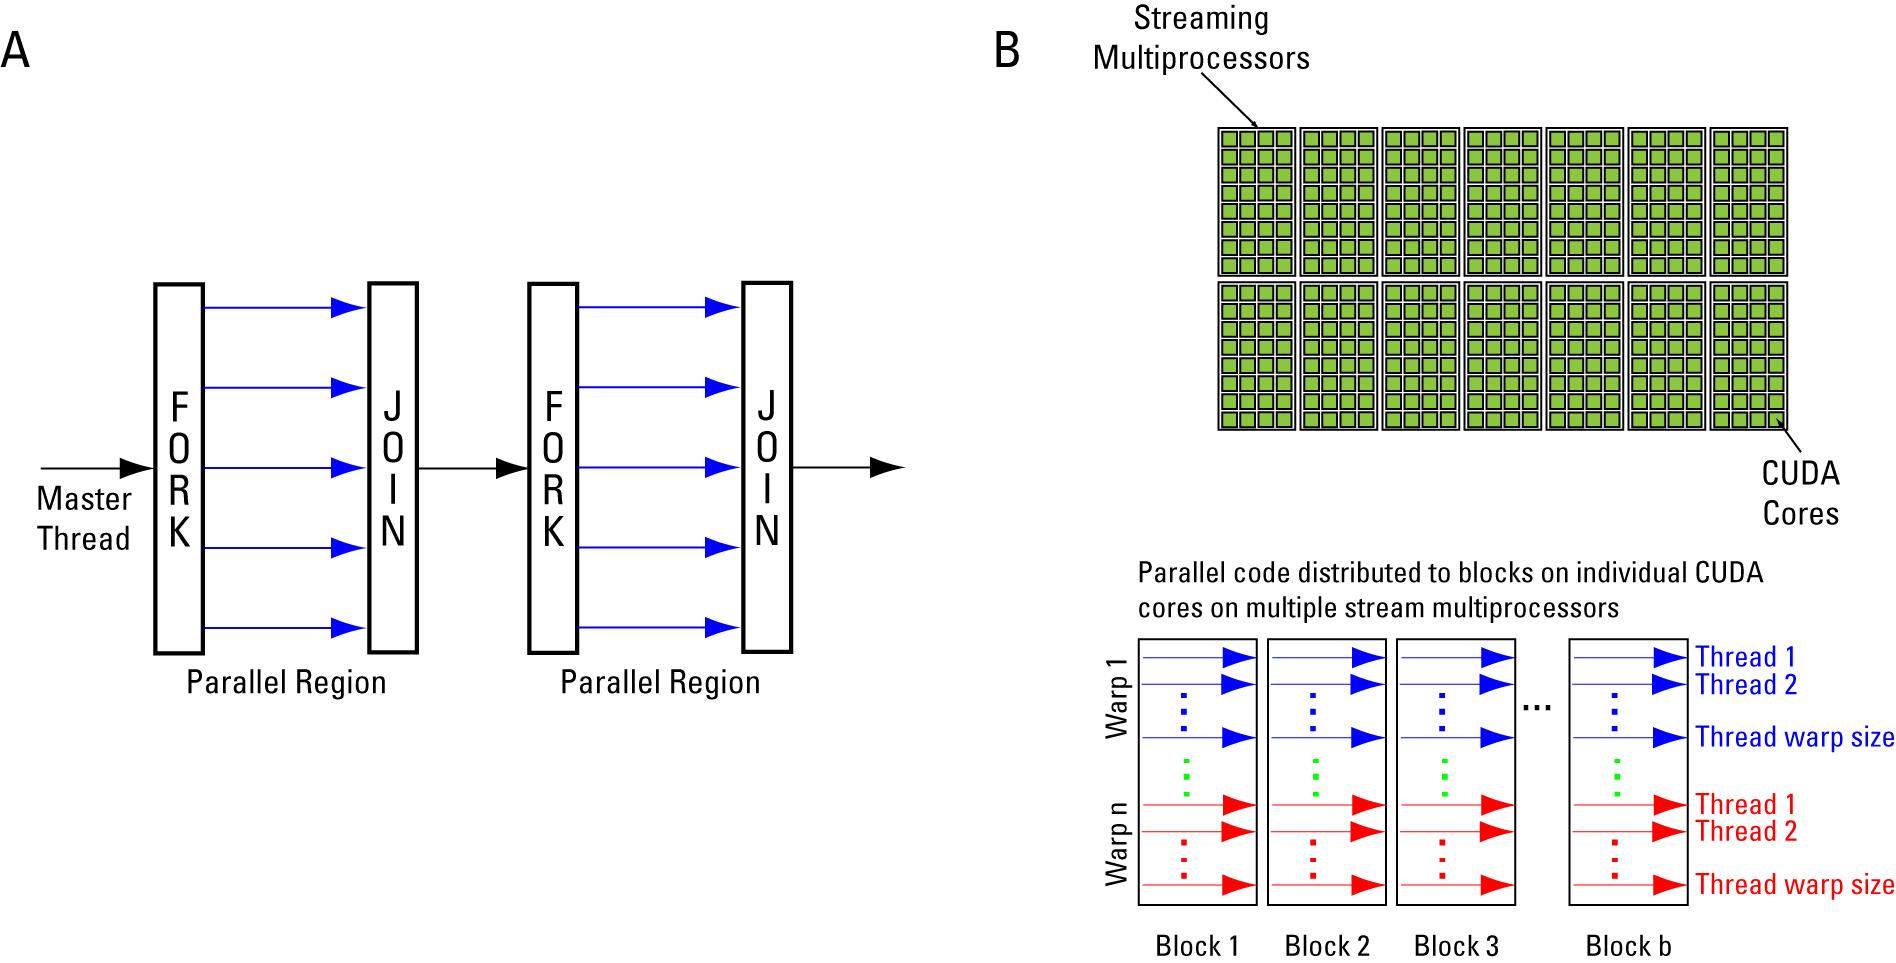
\includegraphics[width=17.15cm]{Figure1.png}
	\caption{(A) Fork-join parallel model. The master thread executes sequential operations and initiates thread forks used in parallel regions. (B) GPGPU architecture showing the relation of streaming multiprocessors and CUDA cores. The fork-join parallel model is applied to blocks of code being executed by thread processing units on multiple streaming multiprocessors.}
	\label{FigParallel}
\end{figure}

%Figure 2
\newpage
\begin{figure}[hp]
	\centering
  	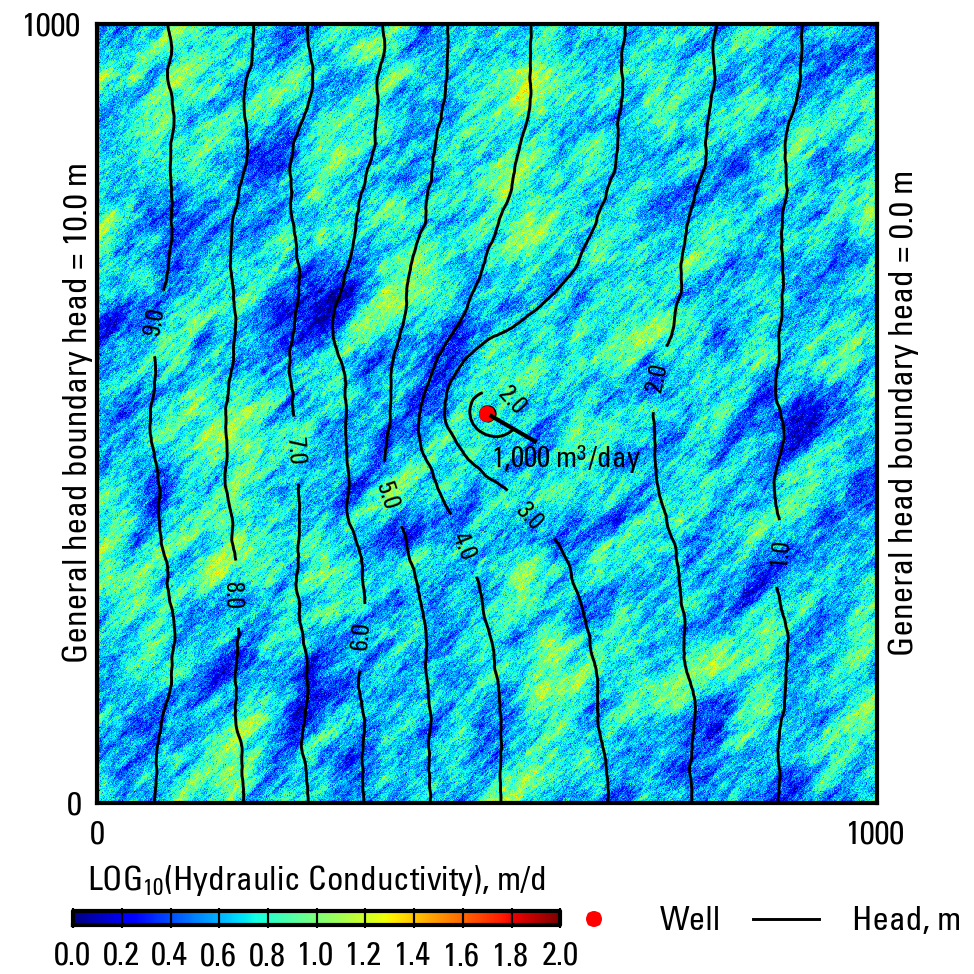
\includegraphics[width=8.25cm]{Figure2.png}
 	\caption{Model domain showing the distribution of hydraulic conductivity and boundary conditions applied to a hypothetical unconfined aquifer. A total of 1,000 m$^{3}$/day are withdrawn from 4 pumping wells. Steady-state groundwater head contours (1 m contour interval) are also shown. Note the effect that groundwater withdrawals and hydraulic conductivity are having on simulated groundwater heads.}
	\label{FigModelDomain}
\end{figure}

%Figure 3
\newpage
\begin{figure}[hp]
	\begin{subfigure}[b]{0.5\textwidth}
		\centering
  		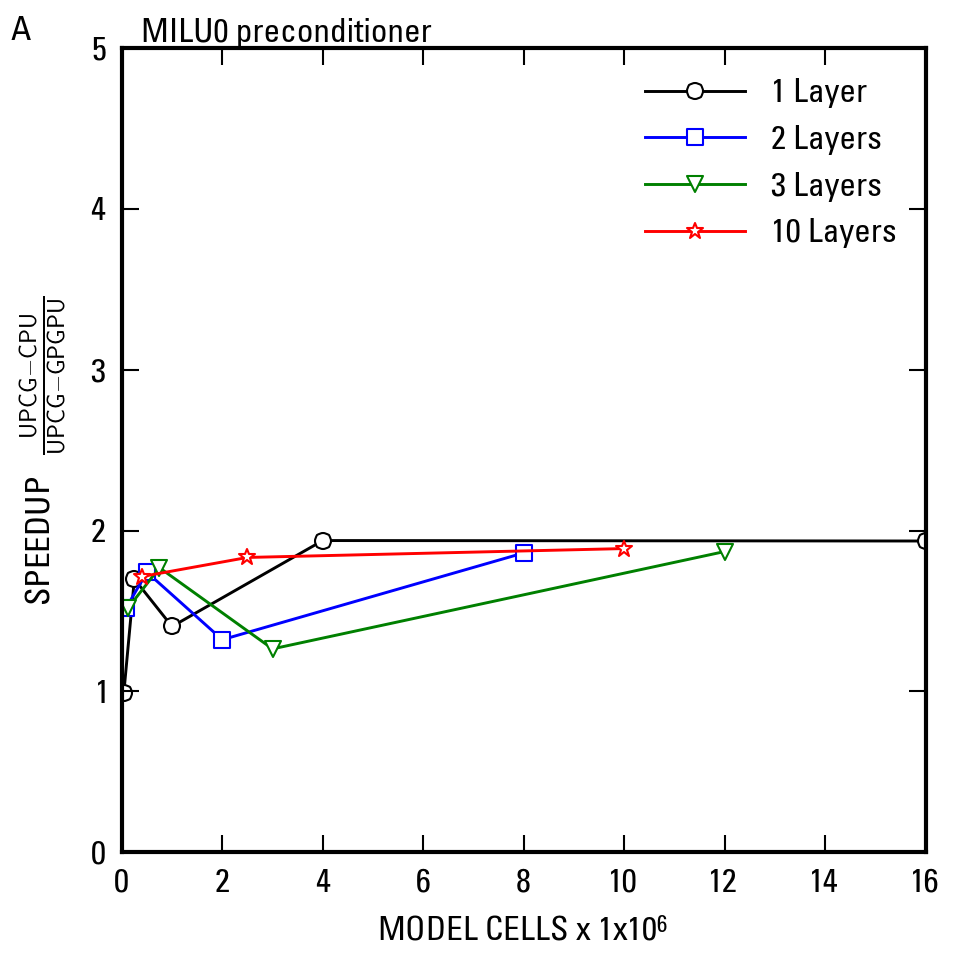
\includegraphics[width=8.25cm]{Figure3a.png}
	\end{subfigure}
	\begin{subfigure}[b]{0.5\textwidth}
		\centering
  		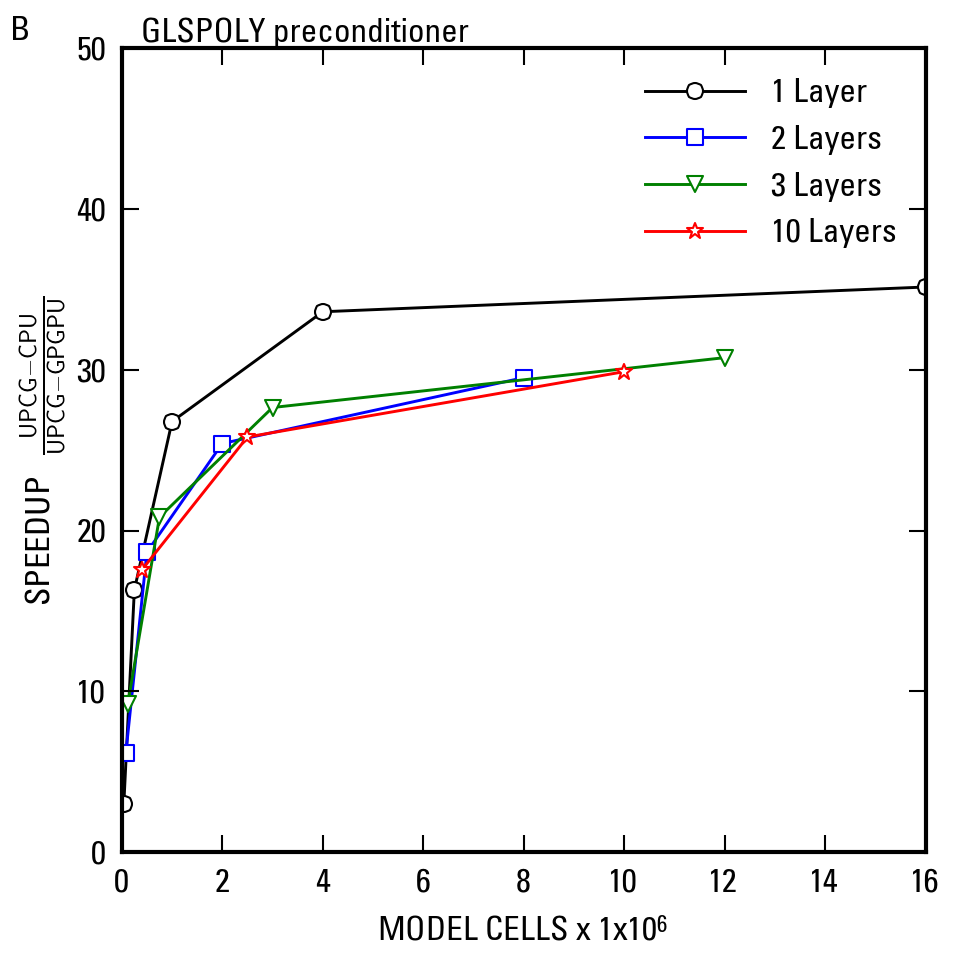
\includegraphics[width=8.25cm]{Figure3b.png}
	\end{subfigure}
 	\caption{Speedup of UPCG solver GPGPU simulations with the (A) MILU0 and (B) GLSPOLY preconditioners relative to sequential UPCG solver simulations executed on the CPU. Note the different scales used for MILU0 and GLSPOLY speedup.}
	\label{FigCPUGPUResults}
\end{figure}

%Figure 4
\newpage
\begin{figure}[hp]
	\begin{subfigure}[b]{0.5\textwidth}
		\centering
  		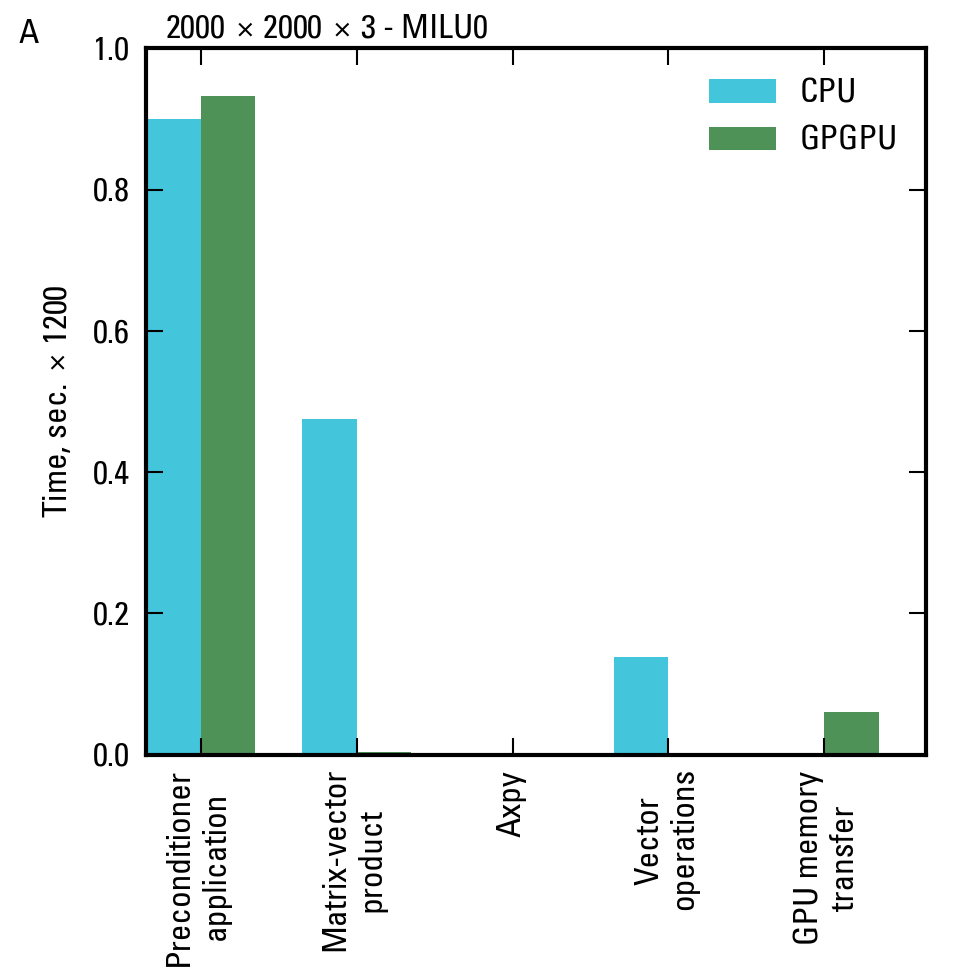
\includegraphics[width=8.25cm]{Figure4a.png}
	\end{subfigure}
	\begin{subfigure}[b]{0.5\textwidth}
		\centering
  		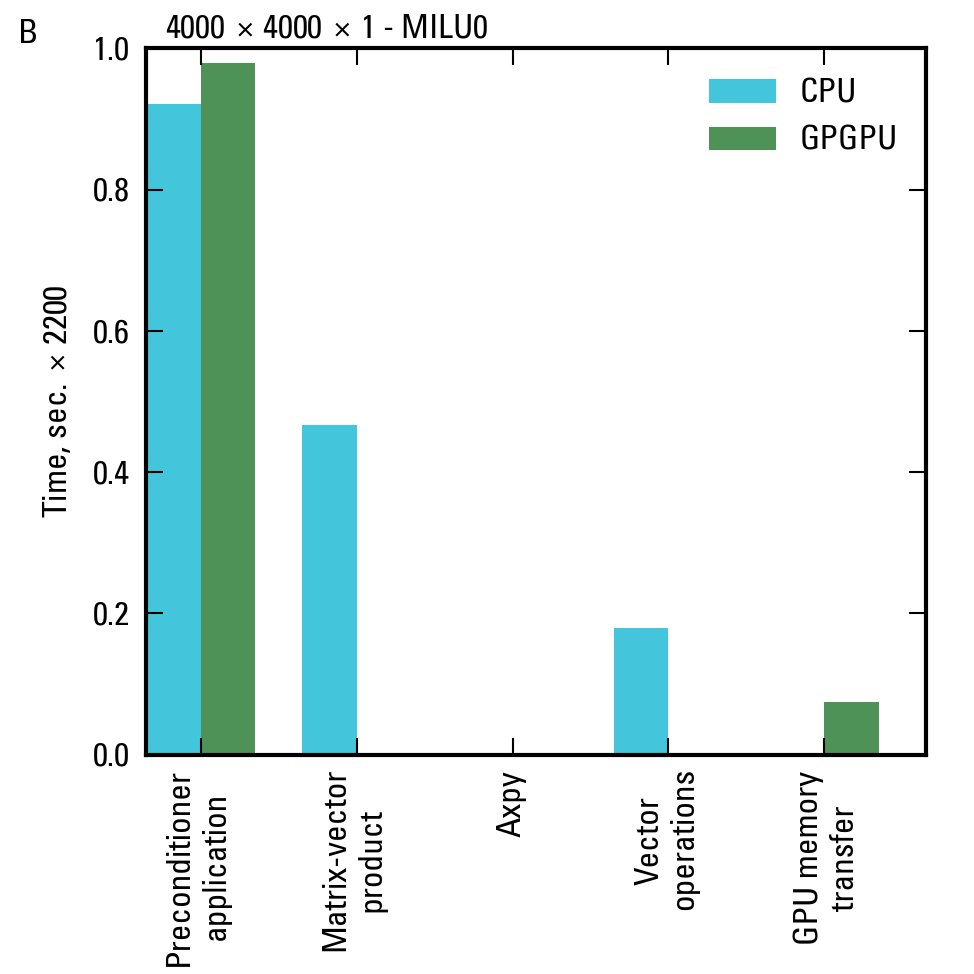
\includegraphics[width=8.25cm]{Figure4b.png}
	\end{subfigure}
	\begin{subfigure}[b]{0.5\textwidth}
		\centering
  		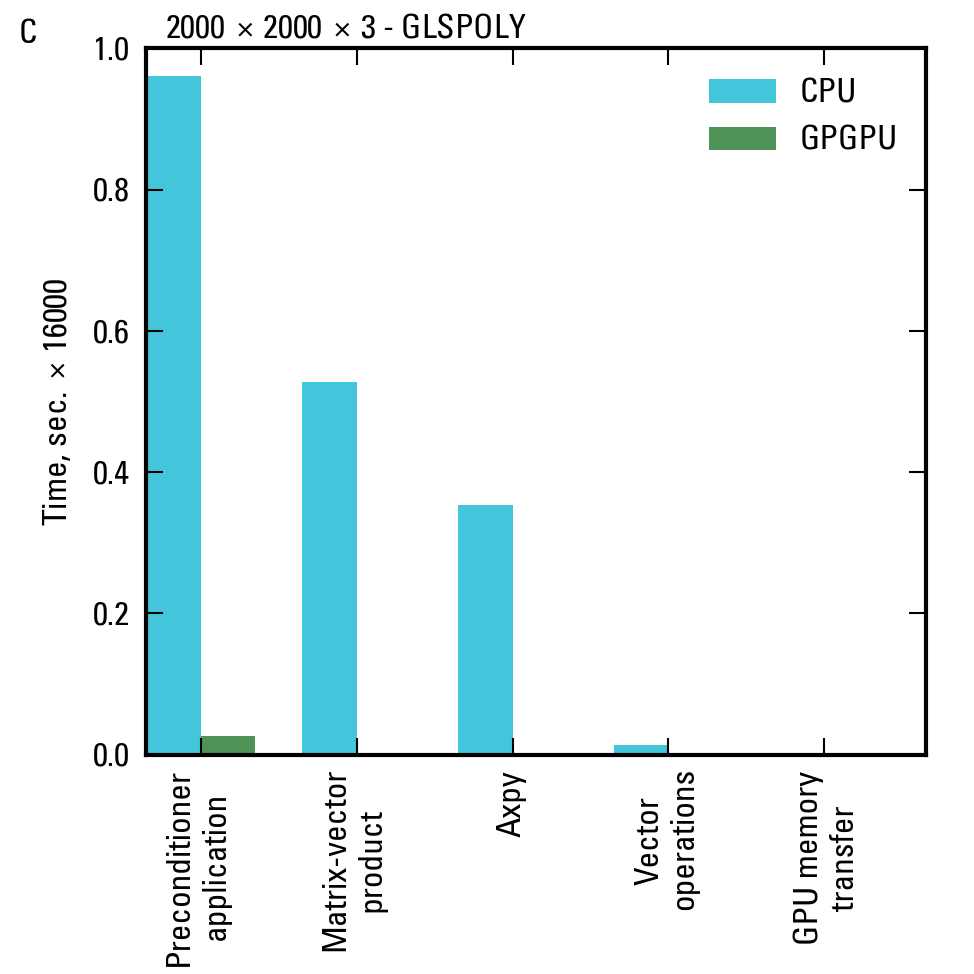
\includegraphics[width=8.25cm]{Figure4c.png}
	\end{subfigure}
	\begin{subfigure}[b]{0.5\textwidth}
		\centering
  		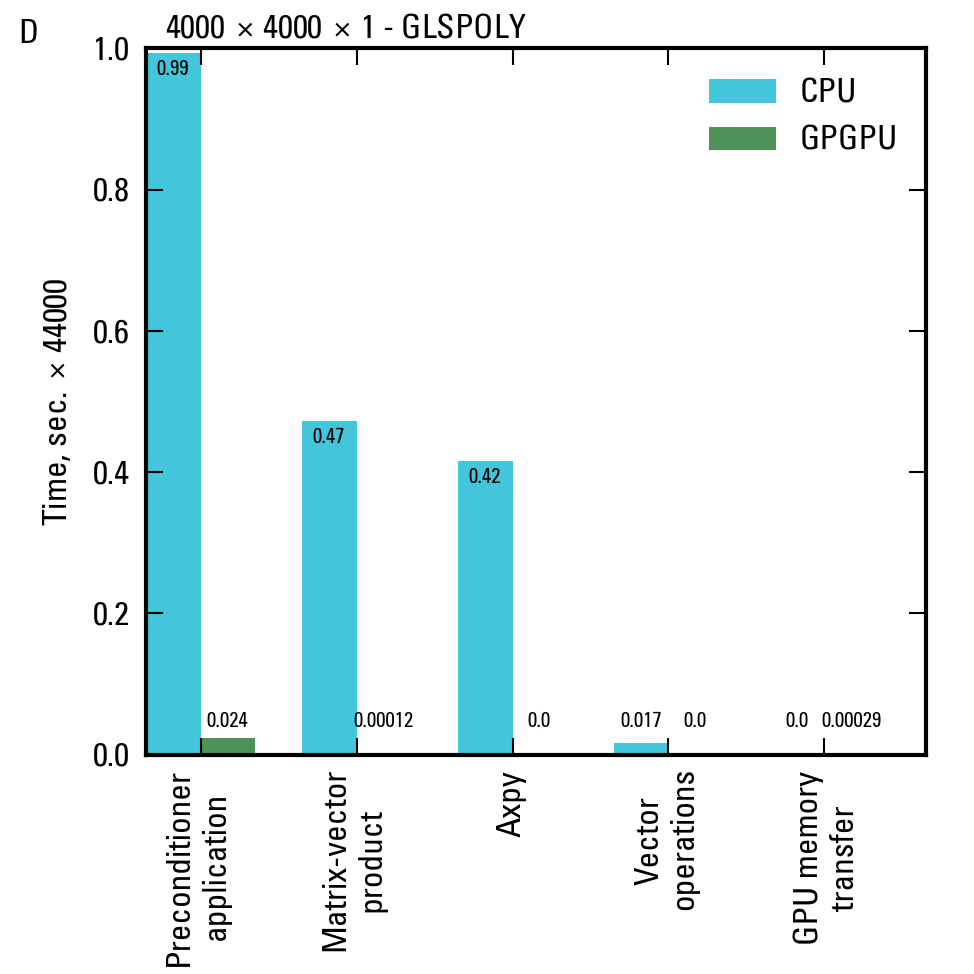
\includegraphics[width=8.25cm]{Figure4d.png}
	\end{subfigure}
 	\caption{Time, in seconds, spent applying the preconditioner, performing BLAS level 1 operations, and transferring data between the CPU and GPGPU for (A) 2,000 $\times$ 2,000 $\times$ 3 problem using the MILU0 preconditioner, (B) 4,000 $\times$ 4,000 $\times$ 1 problem using the MILU0 preconditioner, (C) 2,000 $\times$ 2,000 $\times$ 3 problem using the GLSPOLY preconditioner, and (D) 4,000 $\times$ 4,000 $\times$ 1 problem using the GLSPOLY preconditioner. Note operation execution times have been normalized using the maximum preconditioner application time for each problem to facilitate comparison of different model runs.}
	\label{FigBLASOperationResults}
\end{figure}

%Figure 5
\newpage
\begin{figure}[hp]
	\begin{subfigure}[b]{0.5\textwidth}
		\centering
  		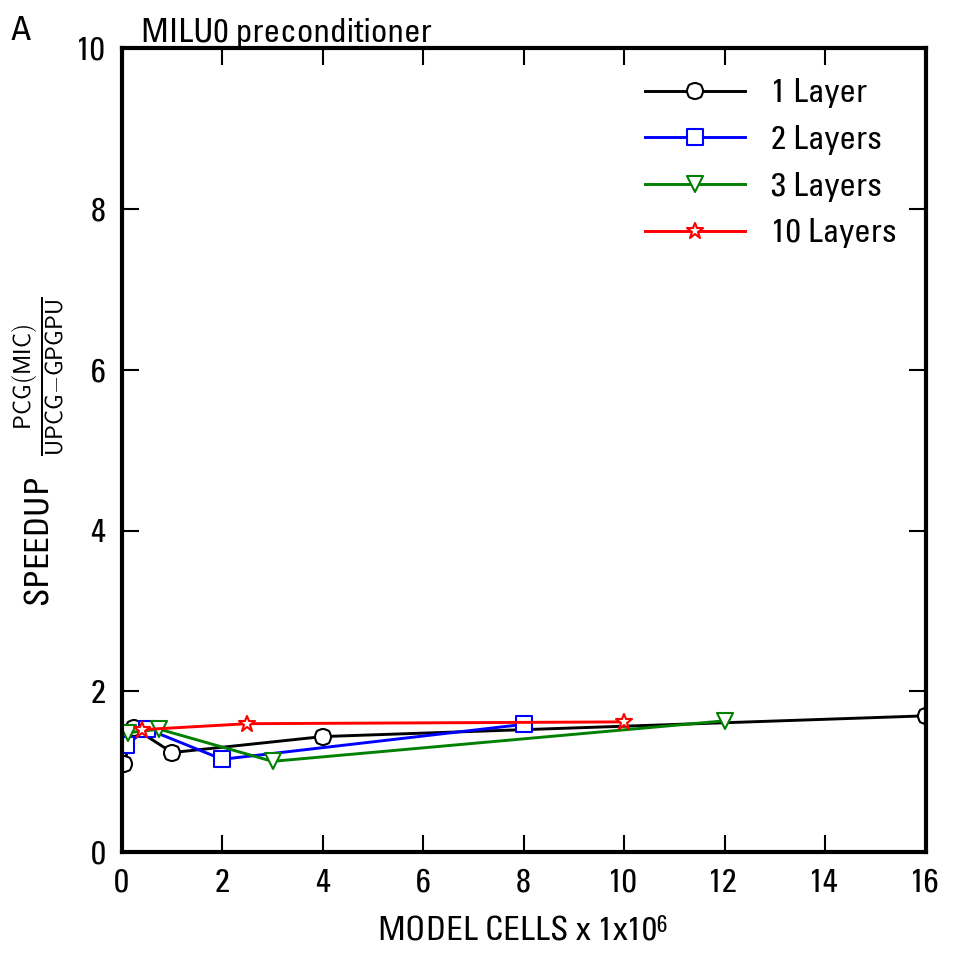
\includegraphics[width=8.25cm]{Figure5a.png}
	\end{subfigure}
	\begin{subfigure}[b]{0.5\textwidth}
		\centering
  		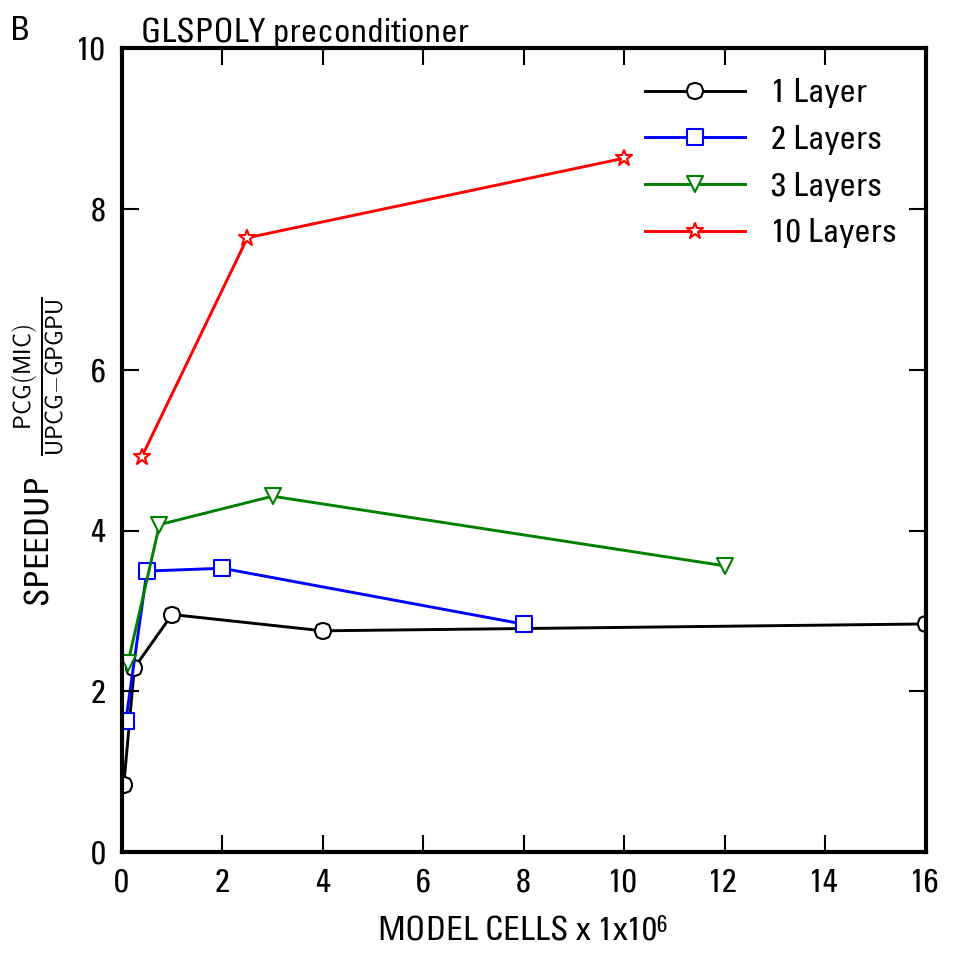
\includegraphics[width=8.25cm]{Figure5b.png}
	\end{subfigure}
 	\caption{Speedup of UPCG solver GPGPU simulations with the (A) MILU0 and (B) GLSPOLY preconditioners relative to simulations performed using the PCG solver with the modified incomplete Cholesky (MIC) preconditioner.}
	\label{FigGPUResults}
\end{figure}

%Figure 6
\newpage
\begin{figure}[hp]
	\centering
  	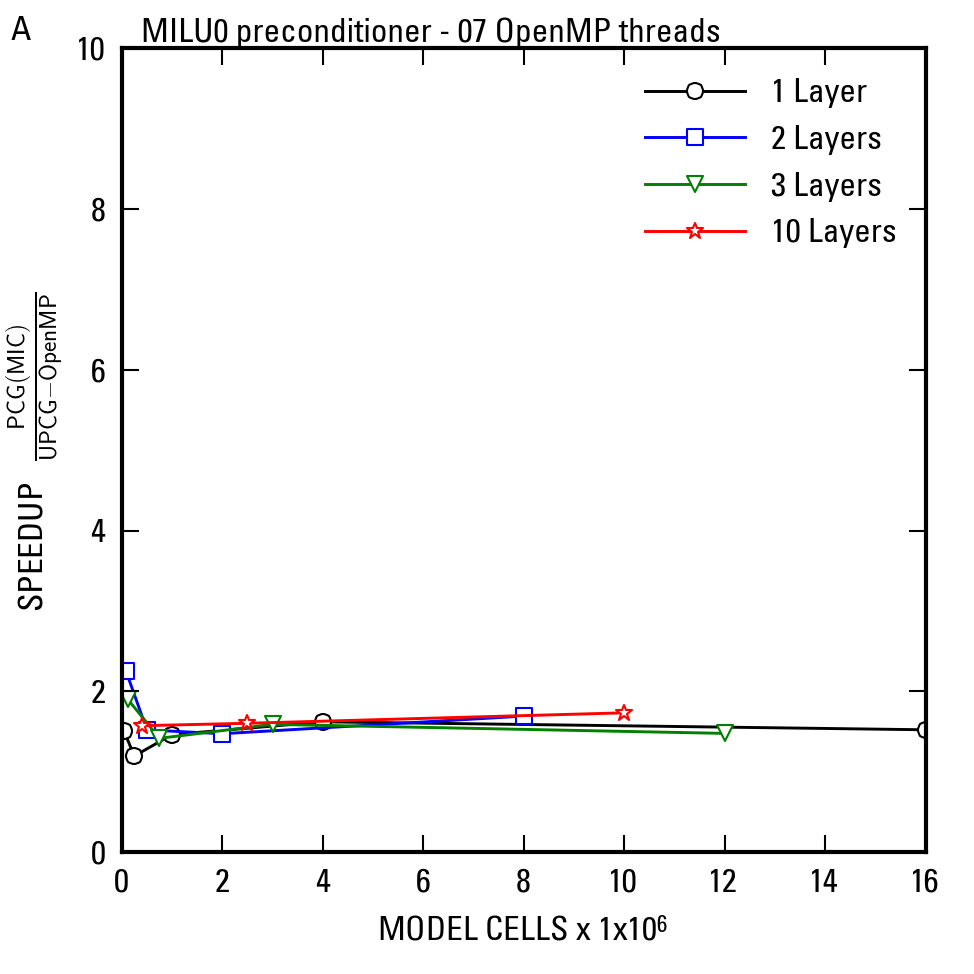
\includegraphics[width=8.25cm]{Figure6.png}
 	\caption{Speedup of parallel CPU simulations using the UPCG solver with the MILU0 preconditioner and 7 threads relative to simulations performed using the PCG solver with the modified incomplete Cholesky (MIC) preconditioner.}
	\label{FigOpenMPResults}
\end{figure}


\end{document}
